%-------------------------------------------------------------------------------
% File: main.tex
%       StockSim project documentation.
%
%       Compile using:
%           $ pdflatex main.tex
%
% Author: Marco Pinna <>
%         Rambod Rahmani <rambodrahmani@autistici.org>
%         Yuri Mazzuoli <>
%         Created on 05/11/2020
%-------------------------------------------------------------------------------
\documentclass[11pt, a4paper, twoside, openright]{book}

% equal left and right margins
\usepackage[hmarginratio=1:1]{geometry}

% configuration to typeset documents in italian
\usepackage[english]{babel}

% include graphics in the file
\usepackage{graphicx}

% used in the dedication environment definition
\usepackage{afterpage}

% used to set page background image
\usepackage{tikz}

\let\cleardoublepage=\clearpage

% blank page command
\newcommand{\blankpage}
{
    \null
    \thispagestyle{empty}%
    \addtocounter{page}{-1}%
    \newpage
}

% dedication environment
\newenvironment{dedication}
{
    % blank page before dedication
    \afterpage{\blankpage}
    % we want a new page
    \clearpage
    % no header and footer
    \thispagestyle{empty}
    % some space at the top
    \vspace*{\stretch{1}}
    % the text is in italics
    \itshape
    % flush to the right margin
    \raggedleft
    % blank page after dedication
    \afterpage{\blankpage}
}
{
    % end the paragraph
    \par
    % space at bottom is one times that at the top
    \vspace{\stretch{1}}
    % finish off the page
    \clearpage
}

\usepackage{color}

\definecolor{pblue}{rgb}{0.13,0.13,1}
\definecolor{pgreen}{rgb}{0,0.5,0}
\definecolor{pred}{rgb}{0.9,0,0}
\definecolor{pgrey}{rgb}{0.46,0.45,0.48}

% Java listings settings
\usepackage{listings}
\lstset{language=Java,
  showspaces=false,
  showtabs=false,
  breaklines=true,
  showstringspaces=false,
  breakatwhitespace=true,
  commentstyle=\color{pgreen},
  keywordstyle=\color{pblue},
  stringstyle=\color{pred},
  basicstyle=\ttfamily,
  moredelim=[il][\textcolor{pgrey}]{$$},
  moredelim=[is][\textcolor{pgrey}]{\%\%}{\%\%}
}
 
\definecolor{dkgreen}{rgb}{0,0.6,0}
\definecolor{gray}{rgb}{0.5,0.5,0.5}
\definecolor{mauve}{rgb}{0.58,0,0.82}
\definecolor{gray}{rgb}{0.4,0.4,0.4}
\definecolor{darkblue}{rgb}{0.0,0.0,0.6}
\definecolor{lightblue}{rgb}{0.0,0.0,0.9}
\definecolor{cyan}{rgb}{0.0,0.6,0.6}
\definecolor{darkred}{rgb}{0.6,0.0,0.0}


\lstset{
  basicstyle=\ttfamily\footnotesize,
  columns=fullflexible,
  showstringspaces=false,
  numbers=left,                   % where to put the line-numbers
  numberstyle=\tiny\color{gray},  % the style that is used for the line-numbers
  stepnumber=1,
  numbersep=5pt,                  % how far the line-numbers are from the code
  backgroundcolor=\color{white},      % choose the background color. You must add \usepackage{color}
  showspaces=false,               % show spaces adding particular underscores
  showstringspaces=false,         % underline spaces within strings
  showtabs=false,                 % show tabs within strings adding particular underscores
  frame=none,                   % adds a frame around the code
  rulecolor=\color{black},        % if not set, the frame-color may be changed on line-breaks within not-black text (e.g. commens (green here))
  tabsize=2,                      % sets default tabsize to 2 spaces
  captionpos=b,                   % sets the caption-position to bottom
  breaklines=true,                % sets automatic line breaking
  breakatwhitespace=false,        % sets if automatic breaks should only happen at whitespace
  title=\lstname,                   % show the filename of files included with \lstinputlisting;
                                  % also try caption instead of title  
  commentstyle=\color{gray}\upshape
}


\lstdefinelanguage{XML}
{
  morestring=[s][\color{mauve}]{"}{"},
  morestring=[s][\color{black}]{>}{<},
  morecomment=[s]{<?}{?>},
  morecomment=[s][\color{dkgreen}]{<!--}{-->},
  stringstyle=\color{black},
  identifierstyle=\color{lightblue},
  keywordstyle=\color{red},
  morekeywords={xmlns,xsi,noNamespaceSchemaLocation,type,id,x,y,source,target,version,tool,transRef,roleRef,objective,eventually}% list your attributes here
}

\usepackage{dirtree}
%-------------------------------------------------------------------------------
% Title page
%-------------------------------------------------------------------------------
\title{
    \vspace{-3cm}
    
\includegraphics[scale=0.3]{img/cherubino_black.eps}\\
    {\scshape University of Pisa}\\
    School of Engineering\\
    \rule{7cm}{0.01cm}\\
    {\normalsize{\scshape Large Scale and Multi-Structured Databases}}\\
    [2cm]
    {\scshape StockSim: Stock Portfolio Simulator}\\
    [3cm]
    \LARGE{\textbf{Supervisor}\hfill\textbf{Students}}\\
    \Large{\emph{Prof. Pietro Ducange}\hfill\emph{Marco Pinna\\}}
    \Large{\hfill\emph{Rambod Rahmani\\}}
    \Large{\hfill\emph{Yuri Mazzuoli\\}}
    \vfill
    \date{\today}
}

% leave the author field ampty in the title page
\author{}

%-------------------------------------------------------------------------------
% Document beginning
%-------------------------------------------------------------------------------
\begin{document}

% make title page
\maketitle

% blank page before dedication
\afterpage{\blankpage}	

% enable page numbering back: roman numbers style
\pagenumbering{roman}

% print table of contents
\tableofcontents

% set arabic page numbering style
\pagenumbering{arabic}

%-------------------------------------------------------------------------------
% Part I: Documentation
%-------------------------------------------------------------------------------
\part{Documentation}
%-------------------------------------------------------------------------------
% File: introduction.tex
%       Part of StockSim project documentation.
%       See main.tex for further information.
%-------------------------------------------------------------------------------
\chapter{Introduction}
StockSim is a Java application which, as main feature, allows users to simulate 
stock market portfolios. The StockSim application is composed by two main 
programs:
\begin{itemize}
    \item \textbf{StockSim Server}: supposed to be running 24/7 to ensure 
            historical data is always up-to-date;
    \item \textbf{StockSim Client}: can be launched in either \texttt{admin} or 
            \texttt{user} mode.
\end{itemize}
The StockSim Server is not thought to be distributed to end users, whereas the 
StockSim Client can be used by both administrators and normal users. The choice 
was made to provide the same program to both administrators and normal users 
with different running modes. Administrators can add new ticker symbols, new 
administrator accounts, delete both administrator and normal user accounts. 
Normal users have access to stocks and ETFs historical data, day by day, 
starting from 2010. They can create their own stock portfolios, run simulations 
a visualize the resulting statistics.\\
\\
Before continuing with what follows, the following terms should be clarified:
\begin{itemize}
    \item
\end{itemize}

%-------------------------------------------------------------------------------
% File: requirements.tex
%       Part of StockSim project documentation.
%       See main.tex for further information.
%-------------------------------------------------------------------------------
\chapter{Actors and requirements}
The main actors and the functional requirements are defined based on the previous
simple description of the application. There is also a 
particular actor which is in charge of the automatic update of the dataset; non-functional
requirements are the characteristics that ensure satisfactory interaction with users and 
real world utility of the product.

\section{Actors}
Based on the application design, four actors can interact with the system:
\begin{itemize}
    \item A \textbf{Guest user} is someone who is not registered on the application; this actor does not 
own private credentials for the login; in order to exploit the application main functionalities, 
it has to register a new account. The registration it is the only action allowed for a Guest;

    \item A \textbf{Registered user} is someone who is registered on the application; this actor owns
private credentials (username and password) for the login; this actor can login as a user
into the client
application and utilize its main features to watch stocks information, compose portfolios and 
simulate them. 
   
    \item An \textbf{Admin user} is someone who is registered on the application with administration
credentials; this actor can login as an admin into the client and do some maintenance 
operations; these operations includes check the integrity of the entire dataset and add new 
stocks to it;

    \item The \textbf{Data Updater} is a thread running on one server; this thread is supposed to 
be always running, and it is in charge of updating the dataset with the new information coming from 
the stock market daily sessions; it is also in charge of finding and fixing (at list report)
integrity issues.

\end{itemize}

The full use case diagram is provided on chapter 3.
\section{Requirements}

\subsection{Functional requirements}
\begin{itemize}
	\item The user, upon launching the application, should be able to sign-up and sign-in.
	\item The user should be able to search for a ticker and view info about it.
	\item The user should be able to view charts on the history of a ticker.
	\item The user should be able to create and delete portfolios.
	\item The user should be able to add/remove tickers to/from their portfolio.
	\item The user should be able to run simulations on a portfolio.
	\item The user should be able to visualize statistics about a simulation and possibly view charts on them.
	\item Only admins should be able to add new stocks to the database.
	\item Only admins should be able to add other admins.
	\item The software should always provide the most recent data about a ticker.
\end{itemize}

\subsection{Non-functional requirements}
\begin{itemize}
	\item The retrieval of data about tickers and portfolios should be fast.
	\item User password should be stored in a secure way (i.e. hashed).
\end{itemize}

%-------------------------------------------------------------------------------
% File: UML_diagrams.tex
%       Part of StockSim project documentation.
%       See main.tex for further information.
%-------------------------------------------------------------------------------
\chapter{UML diagrams}
Blablabla.

\section{Use Case diagram}

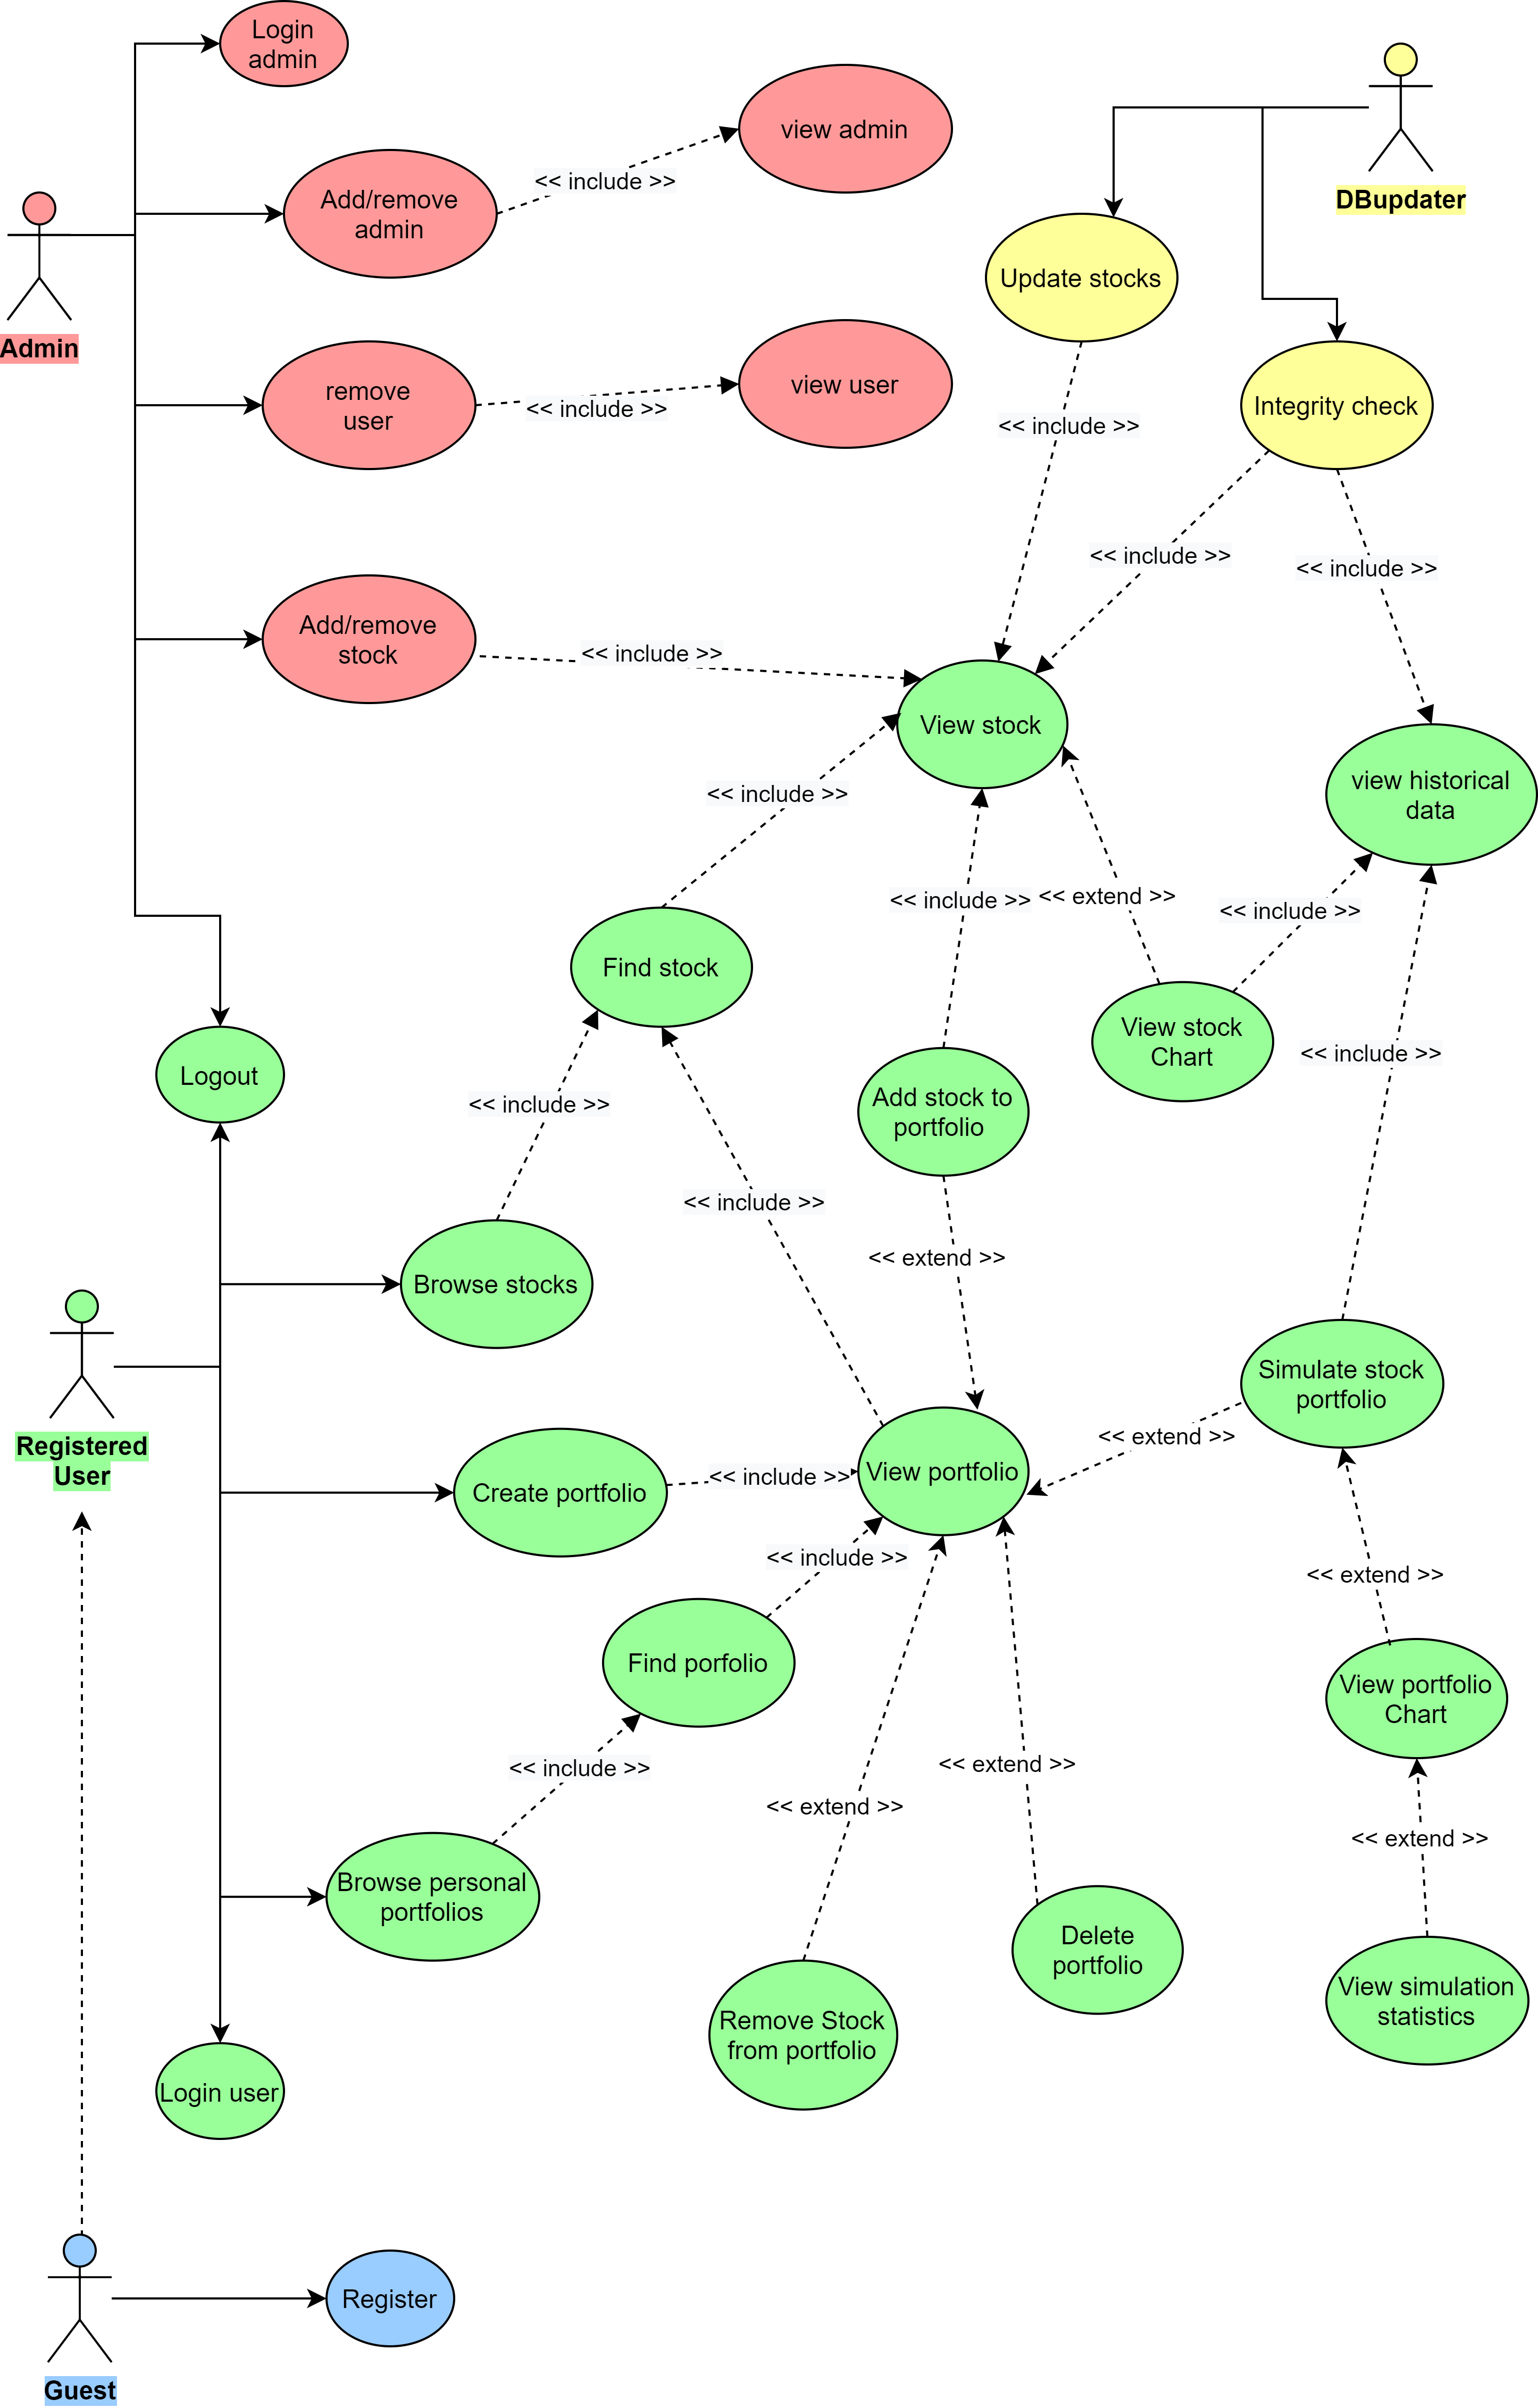
\includegraphics[scale=0.15]{img/use_case.png}

\section{Class diagram}
Something about functional requirements.

%-------------------------------------------------------------------------------
% File: database.tex
%       Part of StockSim project documentation.
%       See main.tex for further information.
%-------------------------------------------------------------------------------
\chapter{Database}
The database is composed by 8235 stocks and ETFs from the US stock market, along
with their general information and historical data; the application also needs to
store users and admins login credentials, personal information and the
composition and details of each user's portfolio.\\
We decided to use a column family database (Apache Cassandra) for the storage of
historical data; this is because historical data represents almost 99\%\ of
the entire database and it is going to be growing very fast as days go by;
aggregation and financial analytics on these volumes of data will perform better
in a column family database where data storage is designed to optimize this type
of operations column by column.\\
We decided to store any other information using a document database (MongoDB),
in order to exploit the schemaless property to save memory; documents frequently
needed together are stored in the same collection and indexes were created to
speed up data retrieval;
\section{Dataset}
The initial set of data was fetched from the web, by means of Python scripts
using the \texttt{pandas}, \texttt{yfinance} and \texttt{JSON} support libraries
and relying upon \url{www.nasdaqtrader.com} and \url{finance.yahoo.com}.
\subsection{NasdaqTrader}
The Nasdaq Stock Market (Nasdaq) is the largest U.S. equities exchange venue by
volume.\\
We choose to take our set of stocks from the Nasdaq index, because it is very
popular and includes a large number of stock, representative of different
economy sectors. This will allow users to interact with big and famous companies
stocks (like Google, Apple, Tesla, etc.) but also to try smaller companies
and/or minor sectors investments. Using NasdaqTrader we fetched the list of
stocks quoted in the NASDAQ index starting from 1970 until today. For each of
the retrieved stock symbol we queried \textbf{Yahoo! Finance} historical
database to populate our own column family database.
\subsection{Yahoo! Finance}
"Yahoo Finance provides free stock quotes, up-to-date news, portfolio management
resources, international market data, social interaction and mortgage rates that
help you manage your financial life."\\
Yahoo Finance is a service, part of the Yahoo network, that provides several of
information about stocks and companies; they are frequently updated, reliable
and well organized.\\
We decided to use this service to retrieve the initial dataset of stocks; we
extract only the fields that we need, and parse into a JSON file. In this way it
is possible to rebuild from scratch this dataset into MongoDB with few commands
(using Python \texttt{mongoimport} support library).\\
With Yahoo Finance it is also possible to retrieve historical data of market
prices for each of the stocks. Using this service it has been possible to build
a dataset of all the market prices of each stocks retrieved from NasdaqTrader;
prices are collected daily, and we decided to take all the values from 2010 to
2020; the obtained dataset (around 1.43 GB) has been parsed to CVS files and then
imported into the Apache Cassandra Cluster. Thanks to the Yahoo Finance service,
it's possible to update every day the database with the last trading session
data. It's also possible to add a new stocks to the dataset, quoted in any
market exchange of any country.
\begin{figure}[H]
	\begin{center}
		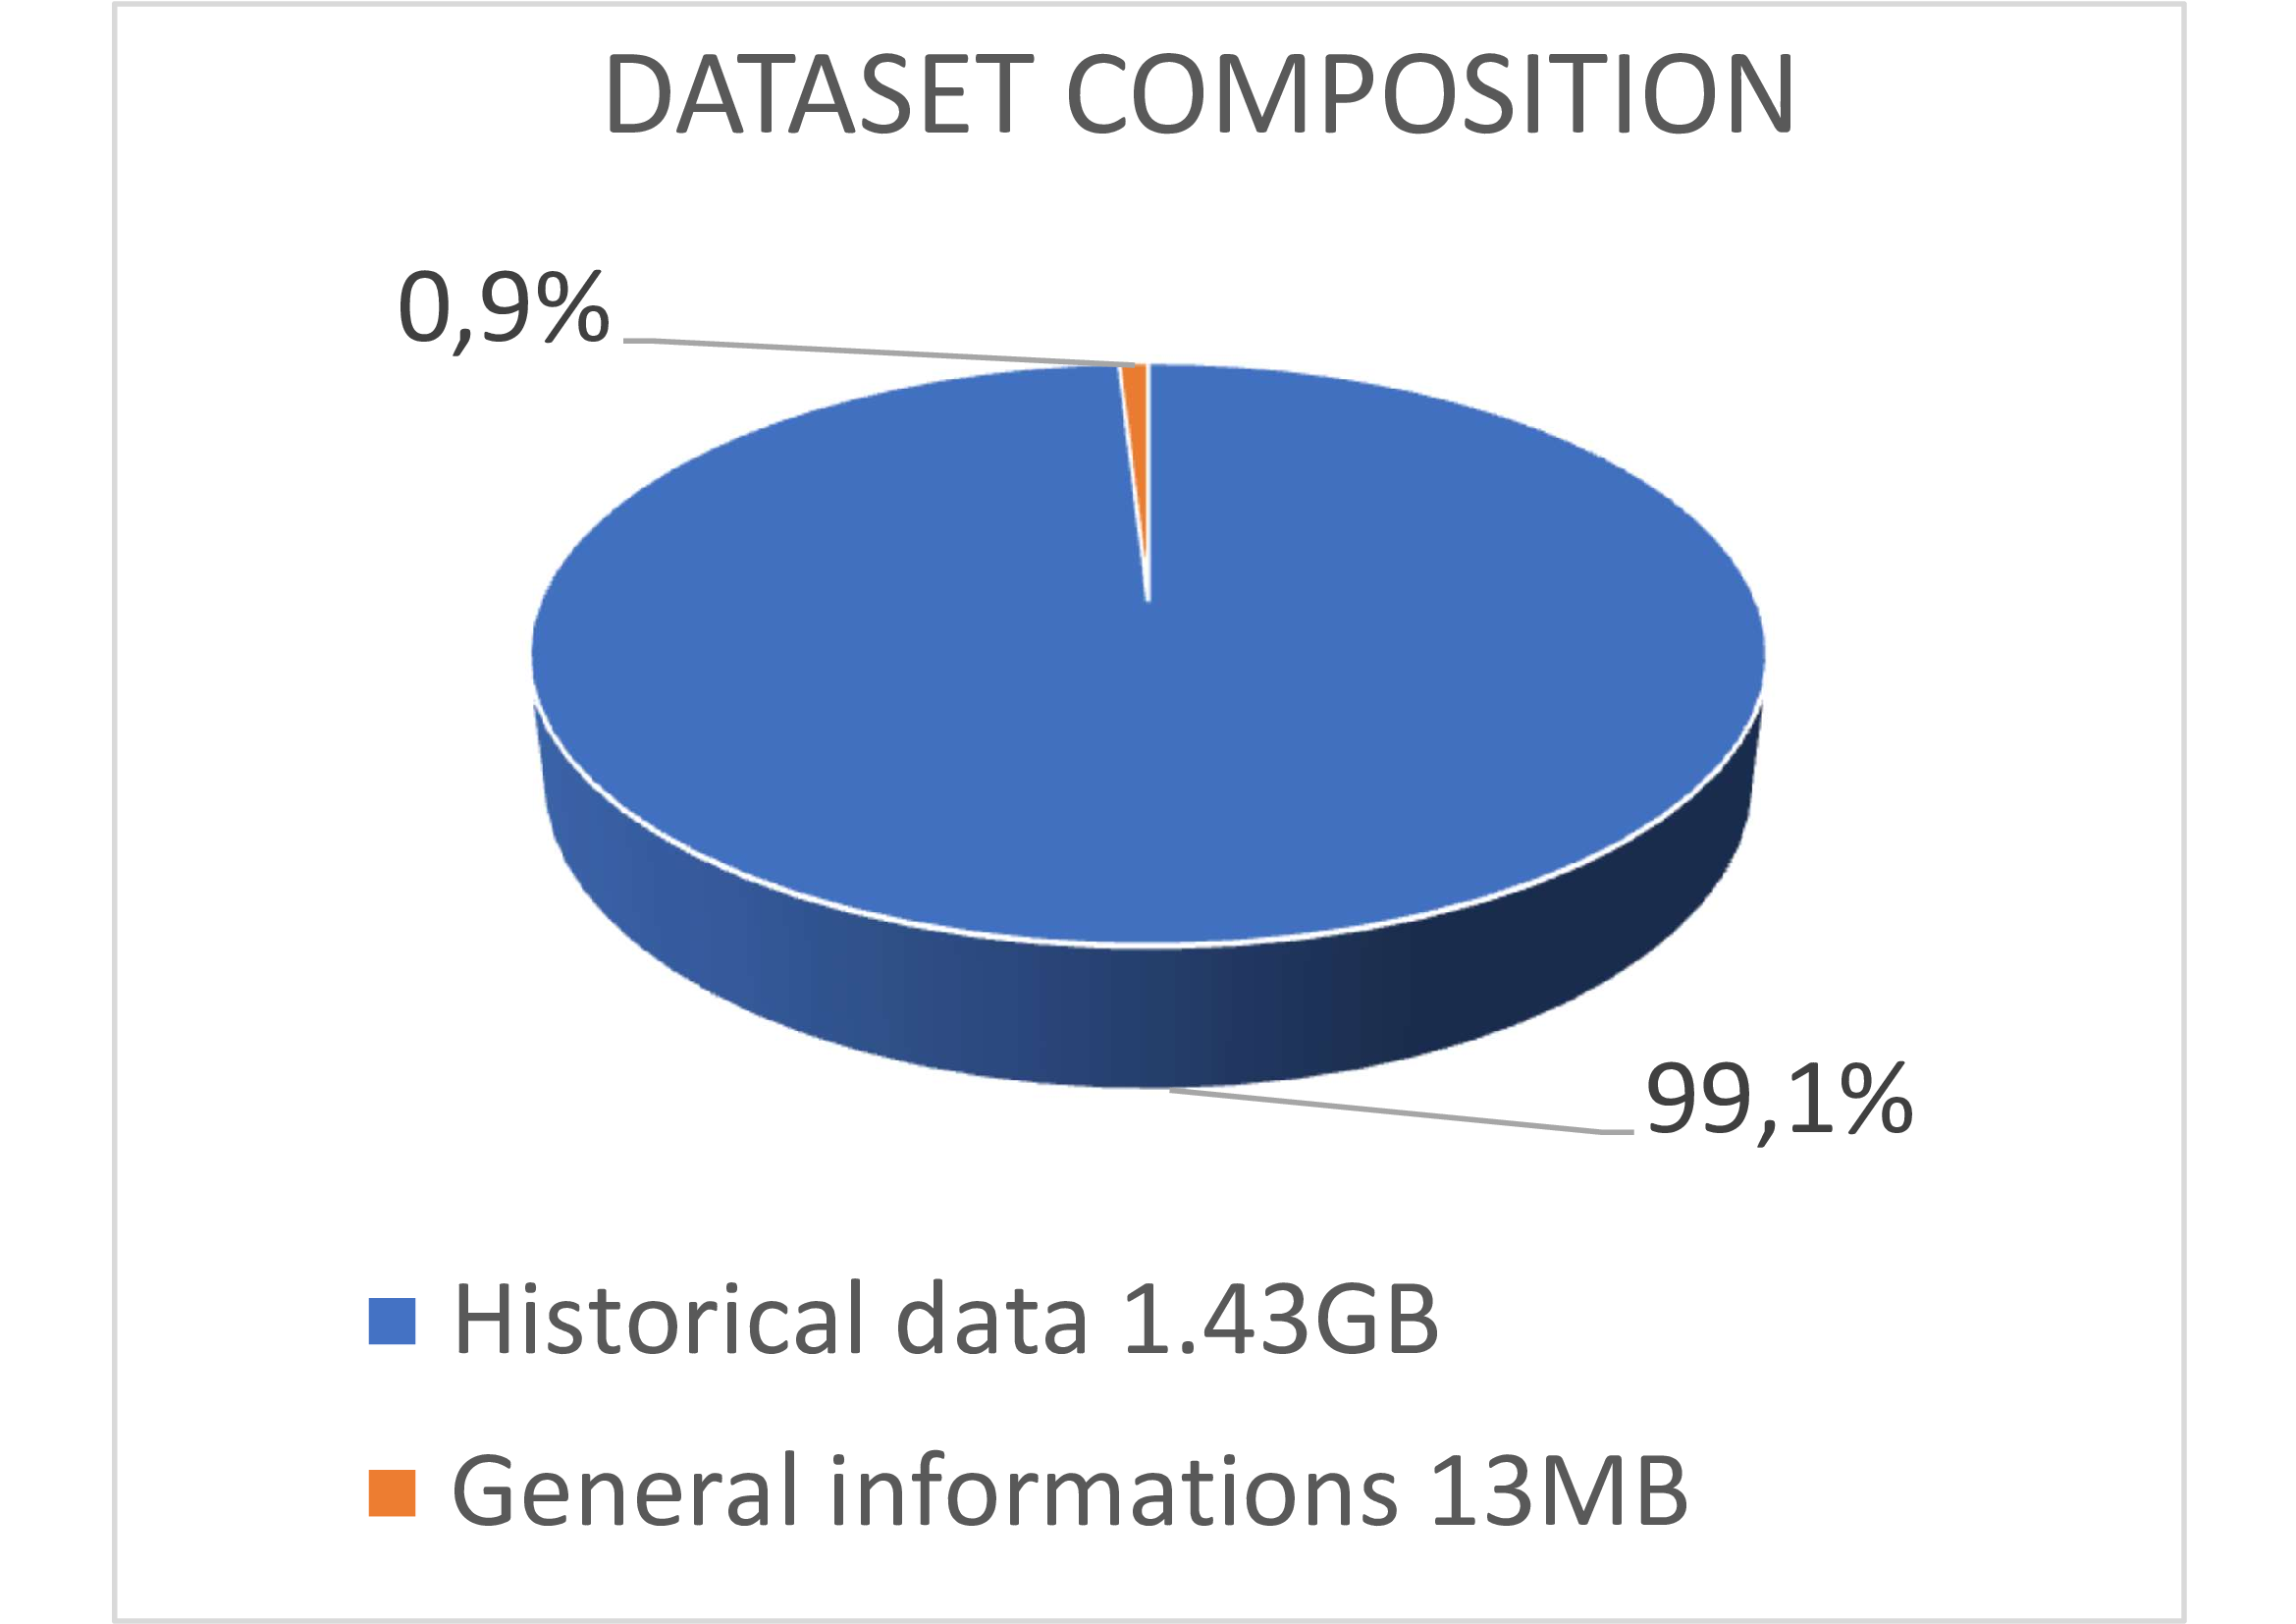
\includegraphics[scale=0.12]{img/dataset_comp.png}
	\end{center}
	\vspace{-0.6cm}
\end{figure}
\noindent
For additional information regarding the implementation of the scripts used to
fetch the raw data please refer to:
\vspace{0.2cm}
\dirtree{%
.1 stocksim/scripts/.
.2 fetch\_db\_content.py.
.2 generate\_cql.py.
.2 merge\_json\_documents.py.
}
\section{MongoDB}
"MongoDB is a general purpose, document-based, distributed database built for
modern application developers and for the cloud era."\\
MongoDB is a very famous document database with a great support for cloud
operations, which will improve the data availability of our application. It also
supports several analytic functions and the creation of custom indexes in order
to speedup read operations.\\
In order to organize data in a meaningful and memory-optimal way, we opted for
this structure:
\begin{figure}[H]
    \vspace{0.2cm}
	\begin{center}
		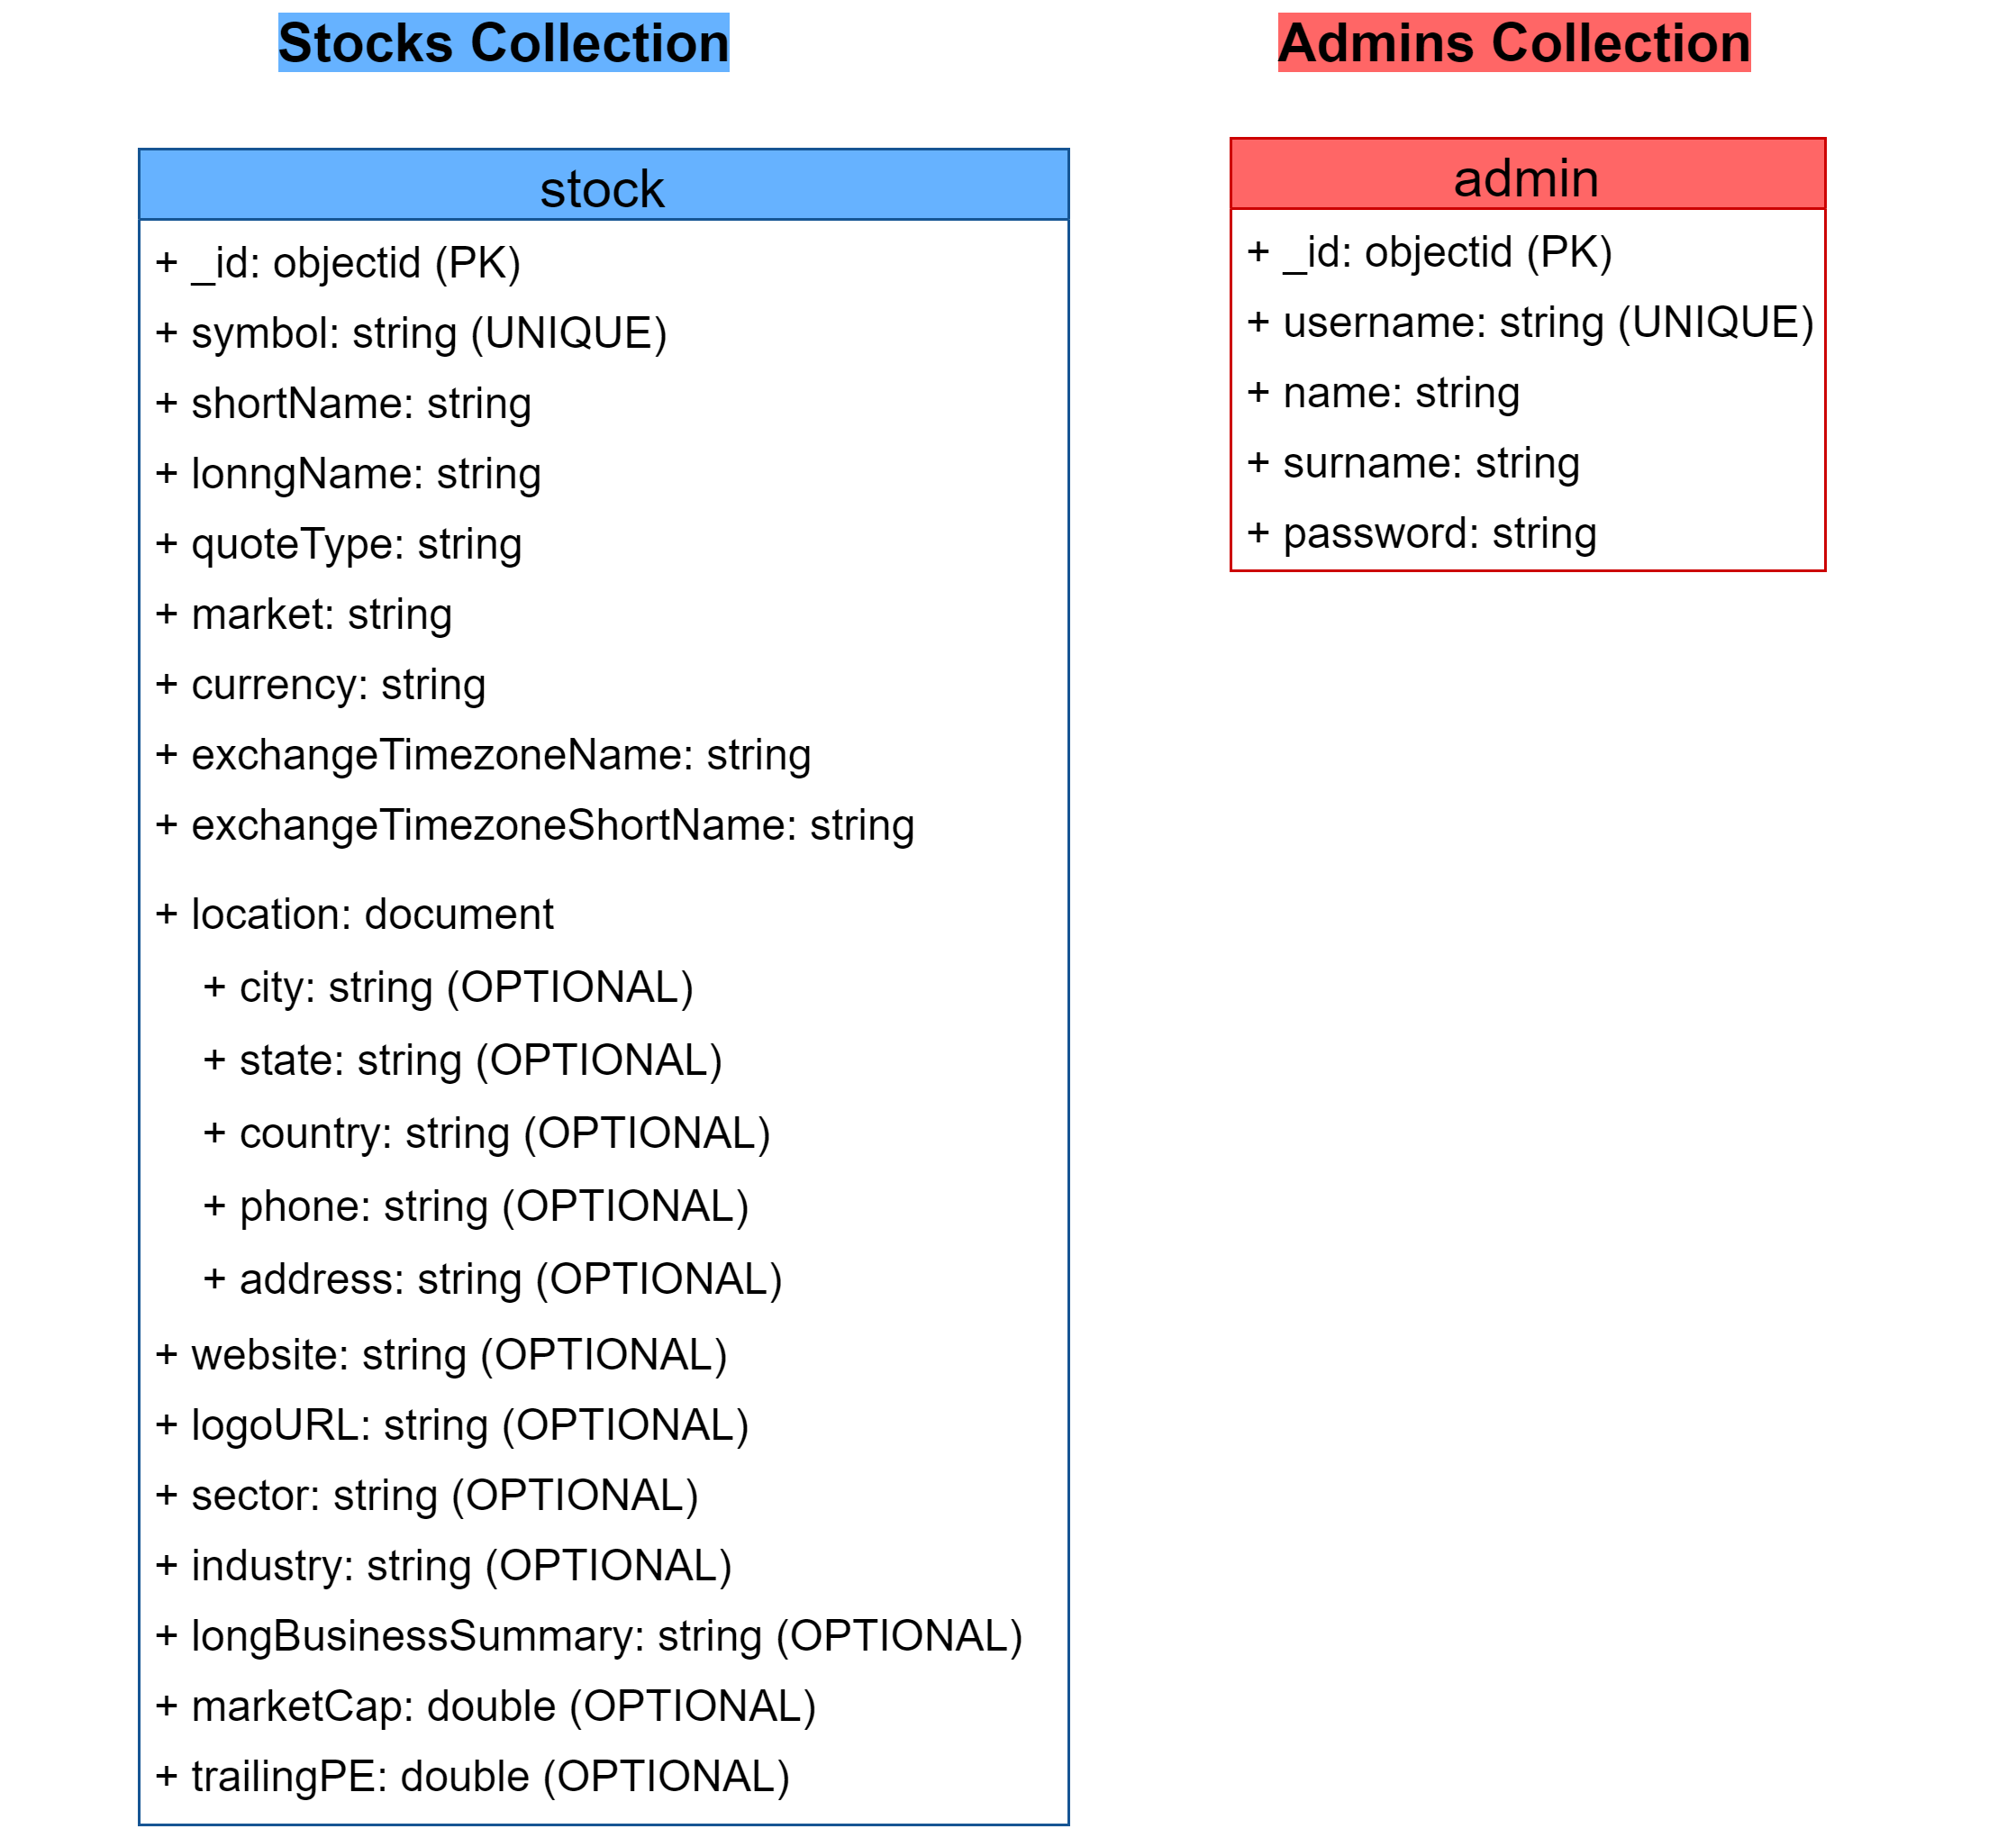
\includegraphics[scale=0.76]{img/mongoDB_schema_1.png}
	\end{center}
\end{figure}
\begin{figure}[H]
	\begin{center}
		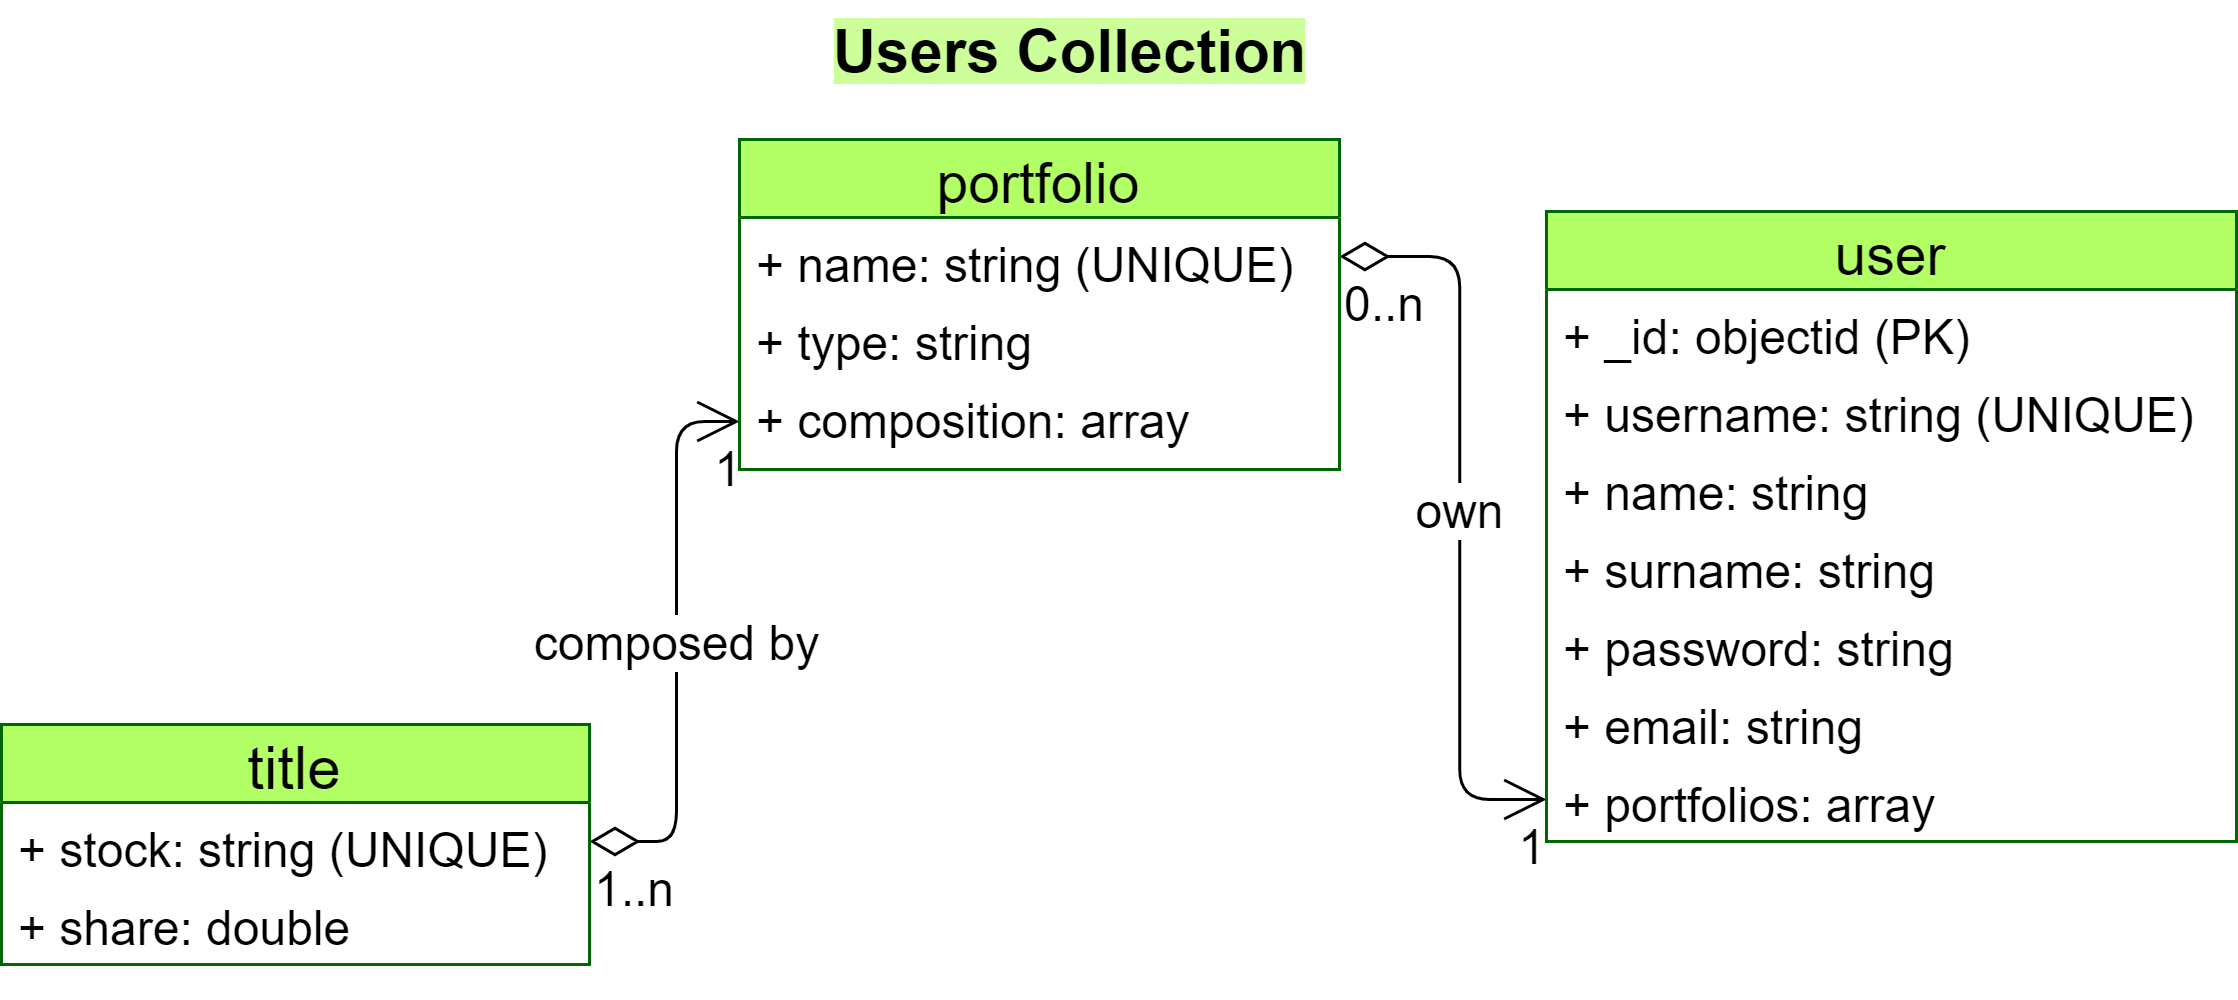
\includegraphics[scale=0.8]{img/mongoDB_schema_2.png}
	\end{center}
\end{figure}
\noindent
This schema is composed by 3 collections: \textbf{stocks}, \textbf{users} and \textbf{admins};
\begin{itemize}
    \item The \textbf{stocks} collection contains one document for each stock;
    inside each document general information about the stock is stored; each
    stock is identified by the attribute \texttt{symbol}; some other basic
    information is always available too, while other may be missing for certain
    stocks; we decided to keep these last type of information were possible,
    exploiting the schemaless property of the document database; available or
    missing attributes have been handled properly Java-side, during the
    implementation;
    \item The \textbf{users} collection contains one document for each user
    registered on the application; in each of these documents, login credentials
    are stored, along with few personal information; for every user there is
    also an array of documents named \texttt{portfolios}: this array contains
    the portfolios of the user; each portfolio has a scheme, which includes an
    array of stocks, named \texttt{composition}, which describes what the
    portfolio consists of; this nested structure has been preferred over
    splitting data in different collections, because all the information of a
    user, including his portfolios, is frequently used all together and fetched
    once; on the other hand, there is no operation that involves portfolios
    owned by different users;
    \item The \textbf{admins} collection contains the admins login credentials
    together with few personal information about them; we decided to create a
    separated collection for administrators to improve the security of the
    administration features: in this way it is impossible to inject
    administration privileges through the login command.
\end{itemize}
\subsection{Aggregations}
One of the main features of our application is the possibility to choose some
stocks from the market and combine them into a portfolio. When a user is looking
for a stock, they want to know statistics about \textbf{industries} and
\textbf{sectors}, along with classification by \textbf{level of capitalization}
and \textbf{P/E ratio} (Price-Earnings Ratio); in order to do so, we will
provide these aggregation pipelines:
\begin{itemize}
    \item the total market capitalization of each sector
    \item the total market capitalization of each industry
    \item the total market capitalization of stocks coming from the same country
    \item the average PE ratio of stocks working in the same sector
    \item the average PE ratio of stocks working in the same industry
    \item the average PE ratio of stocks coming from the same country
    \item the average PE ratio of stocks being in a specific range of market capitalization
\end{itemize}
We provide here an example of an aggregation Mongo query:
\begin{lstlisting}[basicstyle=\footnotesize,language=Java,numbers=left,
    numberstyle=\footnotesize,numbersep=4pt,frame=single]
    /**
    * Aggregates data with filtering and grouping by an attribute, can compute
    * sum, avg ecc.
    *
    * @param collection the collection where to perform the operation;
    * @param filter filter to be used to find the documents.
    * @param groupField the filed used to group the aggregation
    * @param aggregator the aggregator function and field
    *
    * @return iterable object containing the result of the aggregation.
    */
   public AggregateIterable<Document> aggregate(final Bson filter, final String groupField, final BsonField aggregator, final MongoCollection<Document> collection) {
       Bson match = Aggregates.match(filter);
       return  collection.aggregate(
               Arrays.asList(match, Aggregates.group("$"+groupField, aggregator)));
   }
\end{lstlisting}
\begin{lstlisting}[basicstyle=\footnotesize,language=Java,numbers=left,
    numberstyle=\footnotesize,numbersep=4pt,frame=single]
    MongoCollection<Document> collection1 = 
        dbManager.getCollection(
            StocksimCollection.STOCKS.getCollectionName()
        );
    // aggregate examples
    final Bson equity= eq("quoteType", "EQUITY"); //filter(s)
    // name of the field projected, field to accumulate
    // type of accumulation (sum, avg...)
    final BsonField marketCapAccumulator=Accumulators.sum("totalCap","$marketCap");
    AggregateIterable<Document> aggregateList =
                                        // grouping attribute
            dbManager.aggregate(equity, "sector", marketCapAccumulator, collection1);
    for (Document document : aggregateList) {
        System.out.println(document);
    }
    // avg example with nested attribute
    final BsonField PEAccumulator=Accumulators.avg("avgPE","$trailingPE");
    aggregateList =
            dbManager.aggregate(equity, "location.country",
                    PEAccumulator, collection1);
    for (Document document : aggregateList) {
        System.out.println(document);
    }
\end{lstlisting}
\subsection{Indexes}
In order to speed up read operation in the document database, 
we decided to introduce some custom indexes:
\begin{itemize}
    \item a REGULAR and UNIQUE index on the attribute \textbf{symbol} in the collection stocks;
    \item a REGULAR index on the attribute \textbf{marketCAP} in the collection stocks;
    \item a REGULAR index on the attribute \textbf{trailingPE} in the collection stocks;
    \item a REGULAR index on the attribute \textbf{sector} in the collection stocks;
    \item a REGULAR index on the attribute \textbf{industry} in the collection stocks;
    \item a REGULAR index on the attribute \textbf{country} in the collection stocks;
    \item a REGULAR and UNIQUE index on the attribute \textbf{username} in the collection users;
\end{itemize}
We provide some statistic that endorse our indexes choices\\

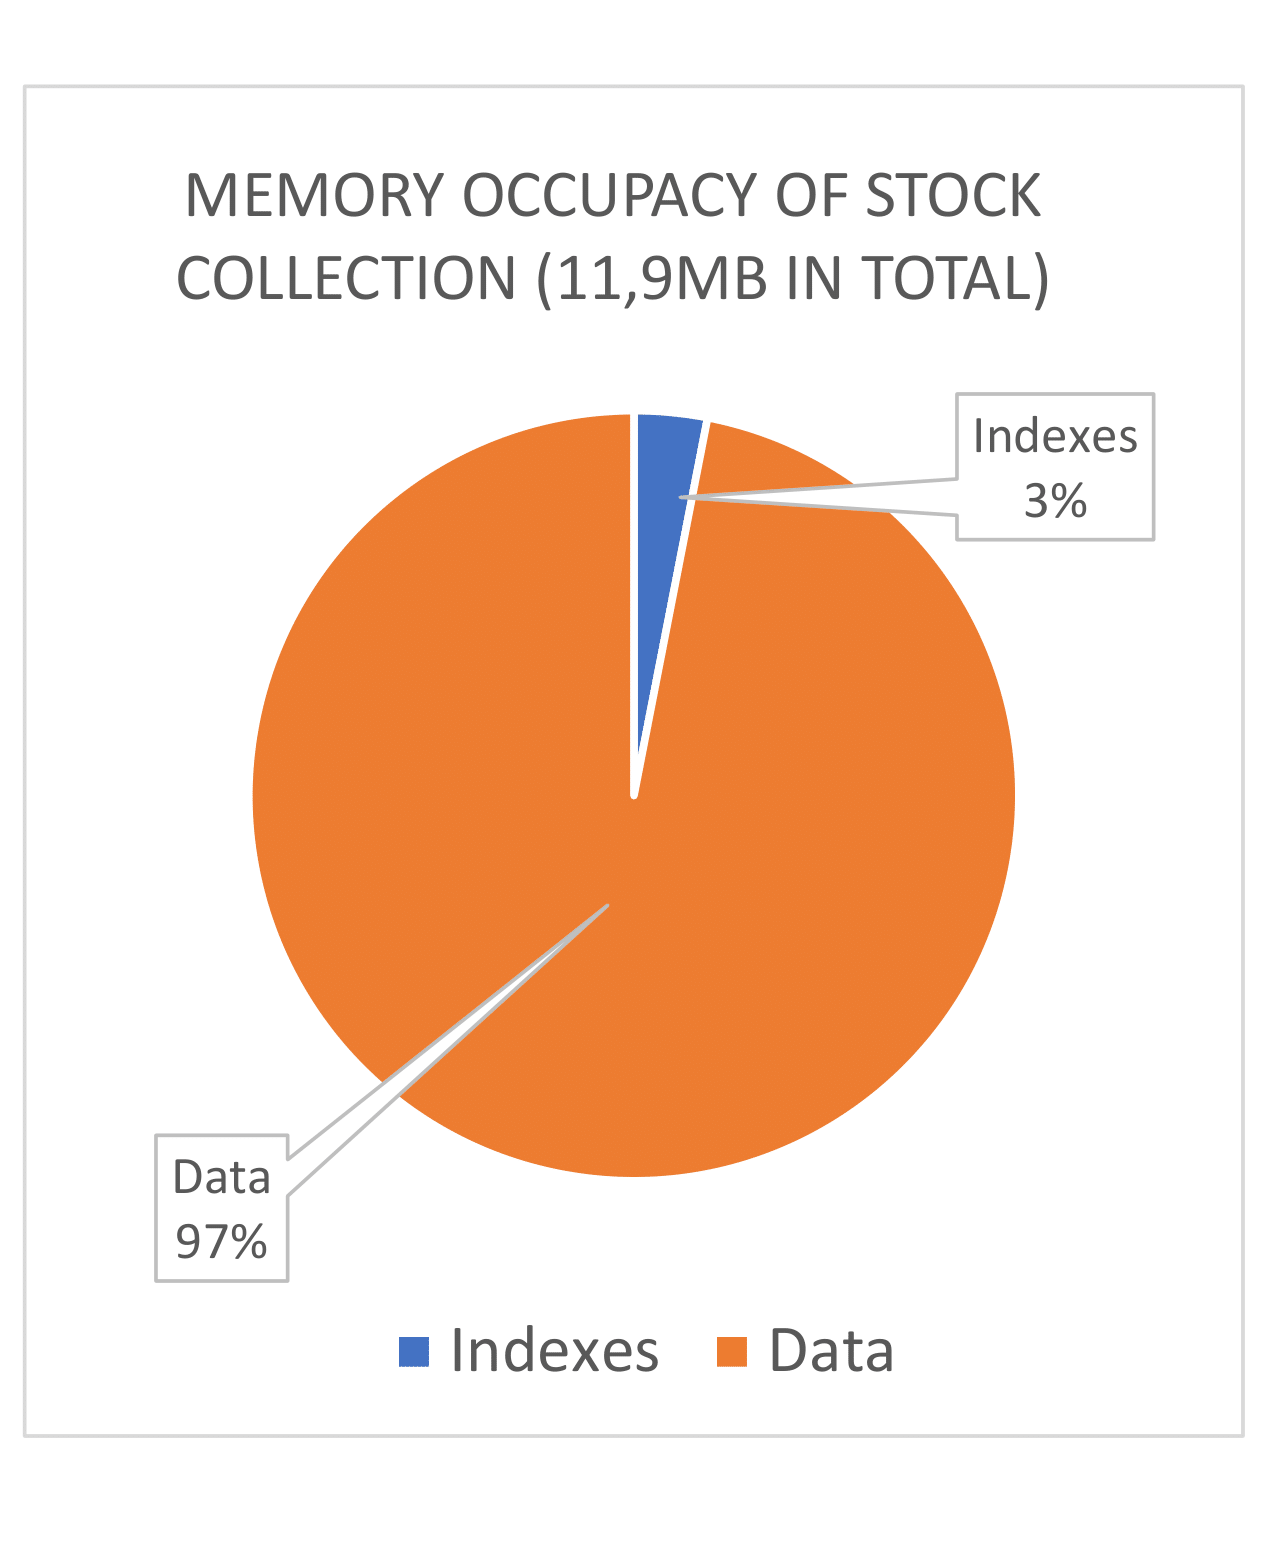
\includegraphics[scale=0.11]{img/memory_mongo.png}
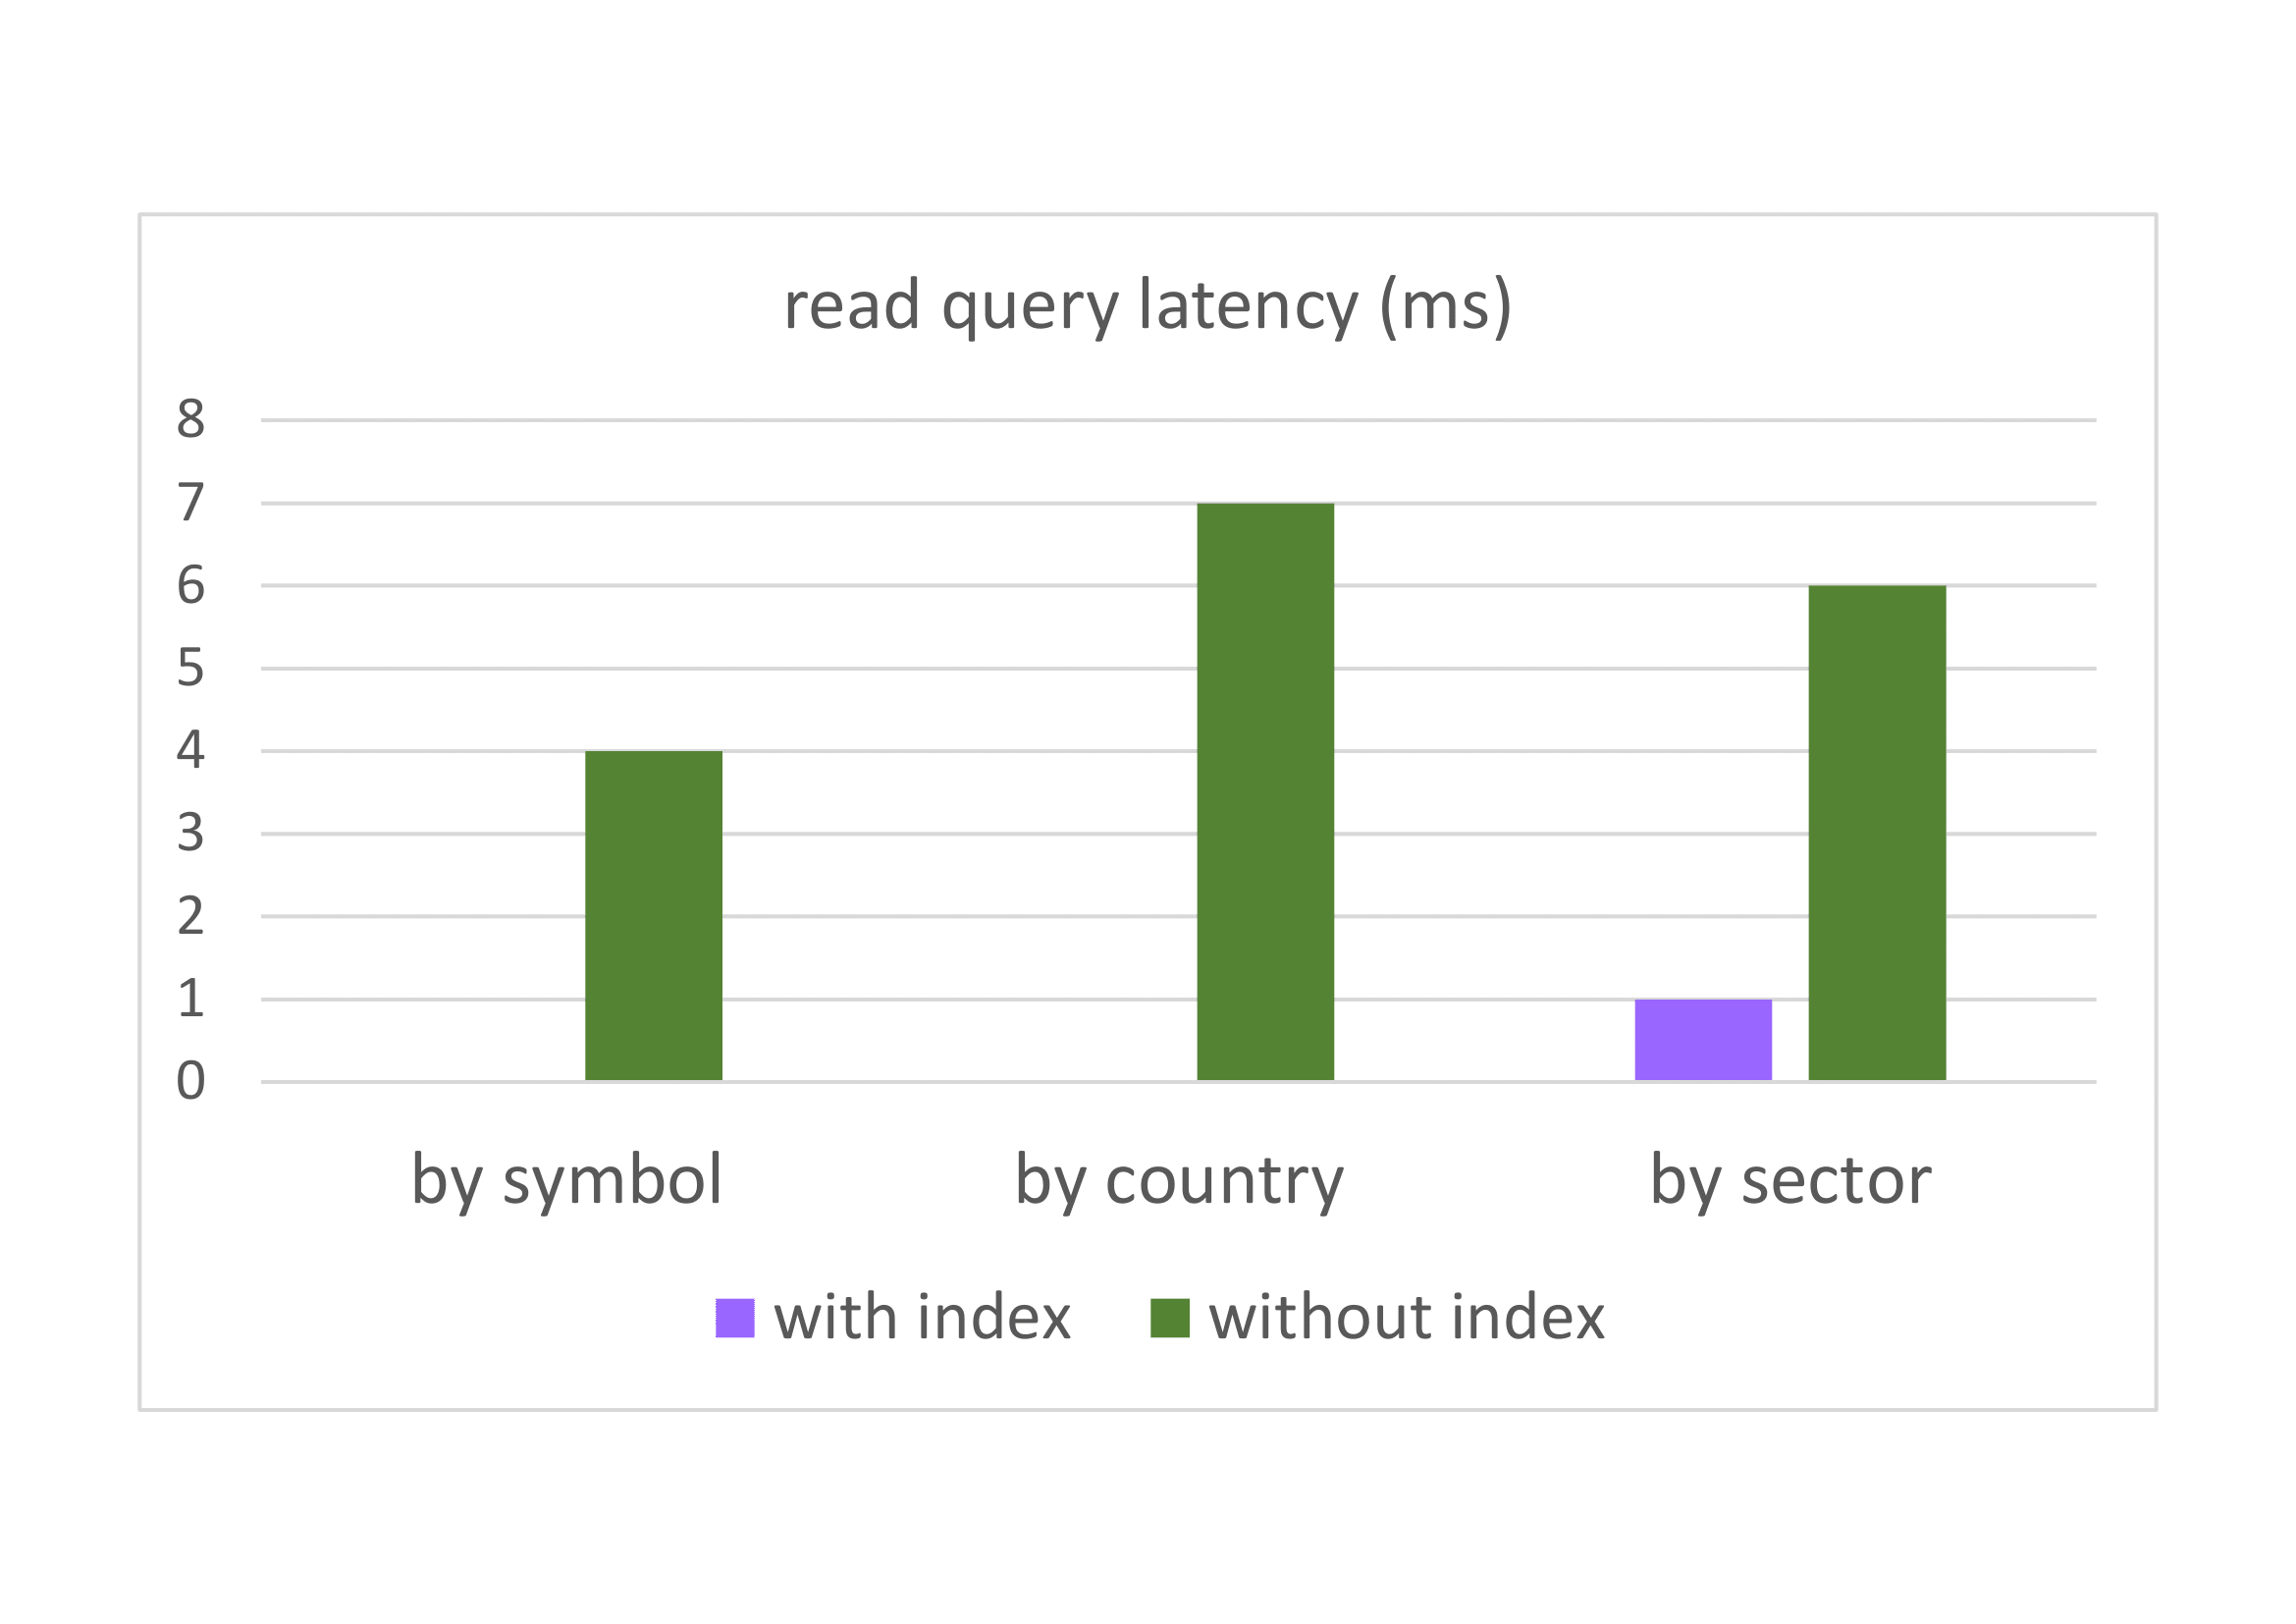
\includegraphics[scale=0.11]{img/latency_mongo.png}\\

\noindent Analog results can be found about the username index in the users collection.

\section{Apache Cassandra}
"The Apache Cassandra database is the right choice when you need scalability and high 
availability without compromising performance. Linear scalability and proven fault-tolerance 
on commodity hardware or cloud infrastructure make it the perfect platform for mission-critical 
data. Cassandra's support for replicating across multiple datacenters is best-in-class, 
providing lower latency for your users and the peace of mind of knowing that you can survive
regional outages." \footnote{https://cassandra.apache.org/}\\
Apache Cassandra is a database designed for high scalability and availability; it is 
capable to handle a huge amount of data and manage it in a decentralized architecture
across multiple nodes. It is built to be write optimized, but with the right indexes choices
read latency can be improved too; tables schemas and analytic functions can be customized.
This is the schema of our Cassandra database:\\
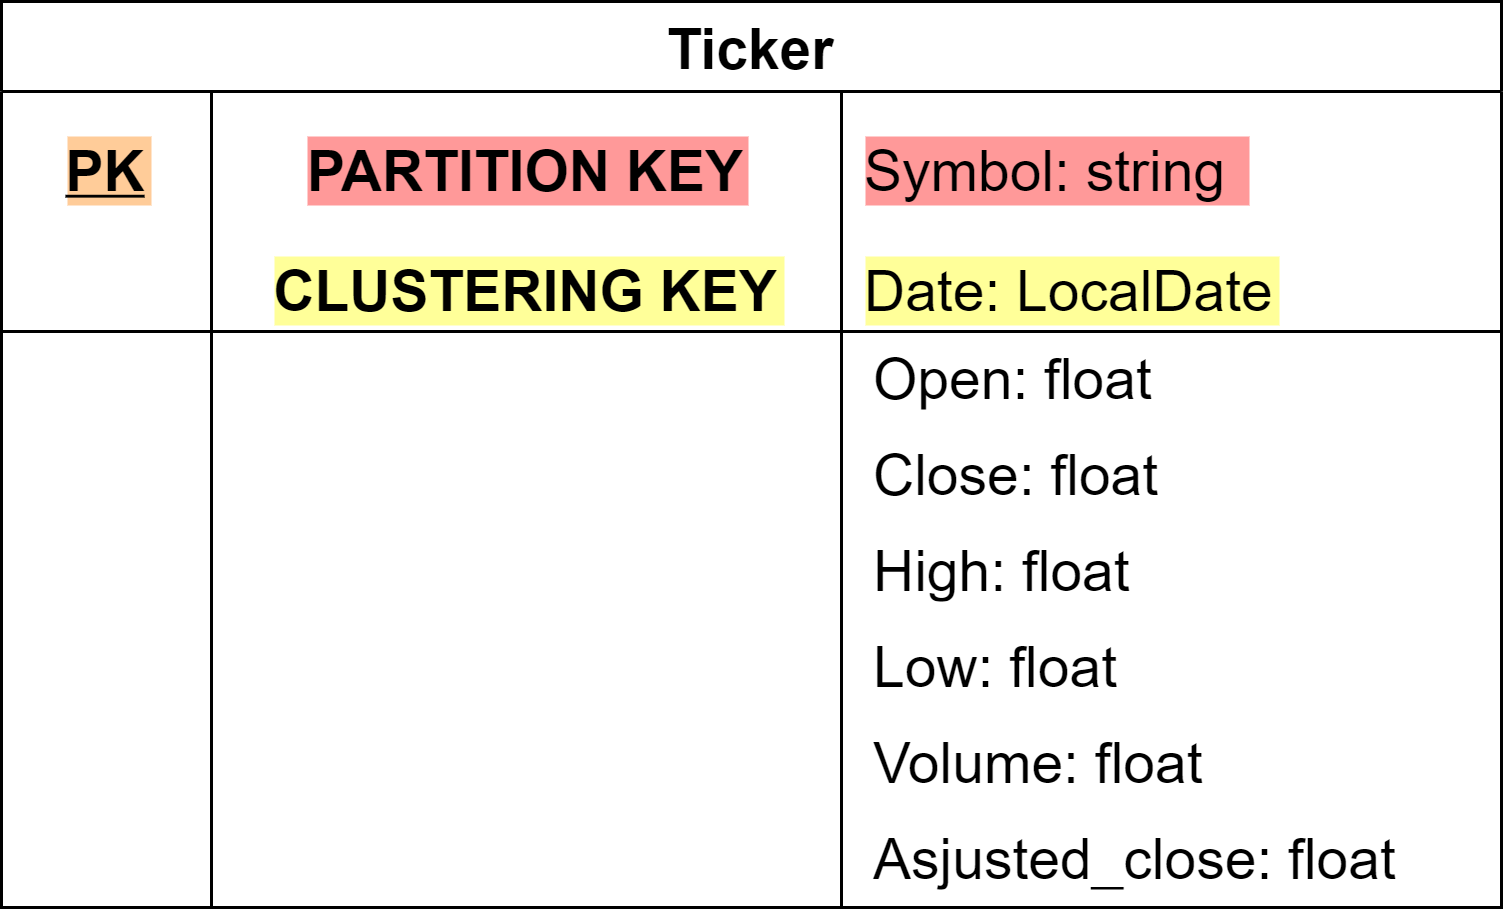
\includegraphics[scale=0.2]{img/cassandraDB_scheme.png}\\

\subsection{Aggregations}
In order to provide snapshots and statistics of stocks and portfolios trends over time,
we exploit the customization functionalities of Cassandra; a custom aggregation has been 
created, specifically to provide aggregate values for periods of time longer than one day; this allows us to obtain customizable granularity for stock market data,
computed on server side; this will not over overwhelm the server, because the aggregator will
execute, for each row, between a memory access and the following. This will greatly reduce
the data to be transmitted from the node to the client, saving bandwidth and time.  \\

\begin{lstlisting}[basicstyle=\footnotesize,language=SQL,numbers=left,
    numberstyle=\footnotesize,numbersep=4pt,frame=single]

    /* State function to be executed for every row*/
    CREATE OR REPLACE FUNCTION PeriodStateParam ( 

    /* the state, containing the aggregation result till this row */
        state map<date,frozen<map<text, float>>>,
    /*  the parameter ndays indicates the duration 
    *   of the period aggregation, in days          */
        ndays int, data date,  
        open float,  close float , high float,  low float, 
        volume float ,  adj_close float)
    CALLED ON NULL INPUT 
    RETURNS map<date,frozen<map<text, float>>> 
    LANGUAGE java AS '
    if (data != null) { 
        int d=0;
        Map<String, Float> statemap=null;
       
        for(d=1; d<ndays;){
            if((statemap=state.get(
                    data.add(Calendar.DAY_OF_MONTH,d)
                ))!=null)
                break;
            d++;
        }
        if(d==ndays){
            statemap=new HashMap<String, Float>();
            statemap.put("open", open);
            statemap.put("close", close);
            statemap.put("high", high);
            statemap.put("low", low);
            statemap.put("volume", volume);
            statemap.put("adj_close", adj_close);
            state.put(data,statemap);
        }
        else{
                if(high>statemap.get("high"))
                    statemap.replace("high", high);
                if(low<statemap.get("low"))
                    statemap.replace("low", low); 
                statemap.replace("volume",statemap.get("volume")+ volume);
                statemap.replace("open",open);
                state.replace(data, statemap); 
        }
    } 
    return state;'
     ;
    
    /*  aggregate declaration
    *   this aggregation generate a map data structure (JSON like):
    *   the key is the end date of each period of nday days, 
    *   and the value is another map containing the aggregate 
    *   values of the period as:
    *        the open of the first day
    *        the close and adjusted close of the last day
    *        the maximum of the highs
    *        the minimum of the lows
    *        the sum of the volumes
    */
    CREATE OR REPLACE AGGREGATE PeriodParam 
        ( int, date,float, float,float, float,float, float ) 
    SFUNC PeriodStateParam
    STYPE map<date,frozen<map<text, float>>>
    INITCOND {}; /* no initial condition is necessary */
    
    /* example of usage, it can be used also with grouping by symbol */
    select PeriodParam(
        20, date, open, close, high, low, volume, adj_close)
        as Period from tickers where 
        date<'2020-12-1' and date>'2020-6-10' 
        and symbol='TSLA';
    
\end{lstlisting}

\subsection{Indexes}
\begin{itemize}
    \item 
The PARTITION KEY index is part of the PRIMARY KEY and it is used to shard the dataset across
the nodes. This index is build on the string symbol, unique for each stock;
    \item
the CLUSTERING KEY i is also part of the PRIMARY KEY, and it is used to maintain rows in
chronological order. This index is built on the attribute date;
\end{itemize}
\section{Sharding and Replicas}
The MongoDB cluster and the Cassandra cluster are deployed on 3 virtual machines provided
by the University of Pisa; 
Our architecture is oriented to the availability of the service and built for the maximum
scalability and decentralization.
\begin{itemize}
    \item 
The Cassandra cluster is built among all 3 nodes, and data is sharded by ticker symbol;
in this way every node stores 1/3 of the main dataset, and aggregation functions are computed
on records that lie in the same node; each node also stores a backup of the data
assigned to another node, giving us a replication factor of 2. There are 2 seed nodes,
which are responsible for the cluster: the cluster is online as long as one of them keeps
working. This is indeed a minor issue, because in any case, with only one node, the dataset 
would by incomplete. The decentralized behaviour of Cassandra ensures that
even if all the node were to go offline, the cluster would return available as soon as one seed server went back
online. 
    \item
The MongoDB cluster is also built among all 3 virtual machines, and the service is replicated;
an initial primary server is elected, then another one will take its place if the former goes down. 
The cluster is available as long as one server is working, and incoming traffic could be balanced
with the "nearest" preference on client connection; in this way the client would connect to the
server with the lowest ping time.

\end{itemize}
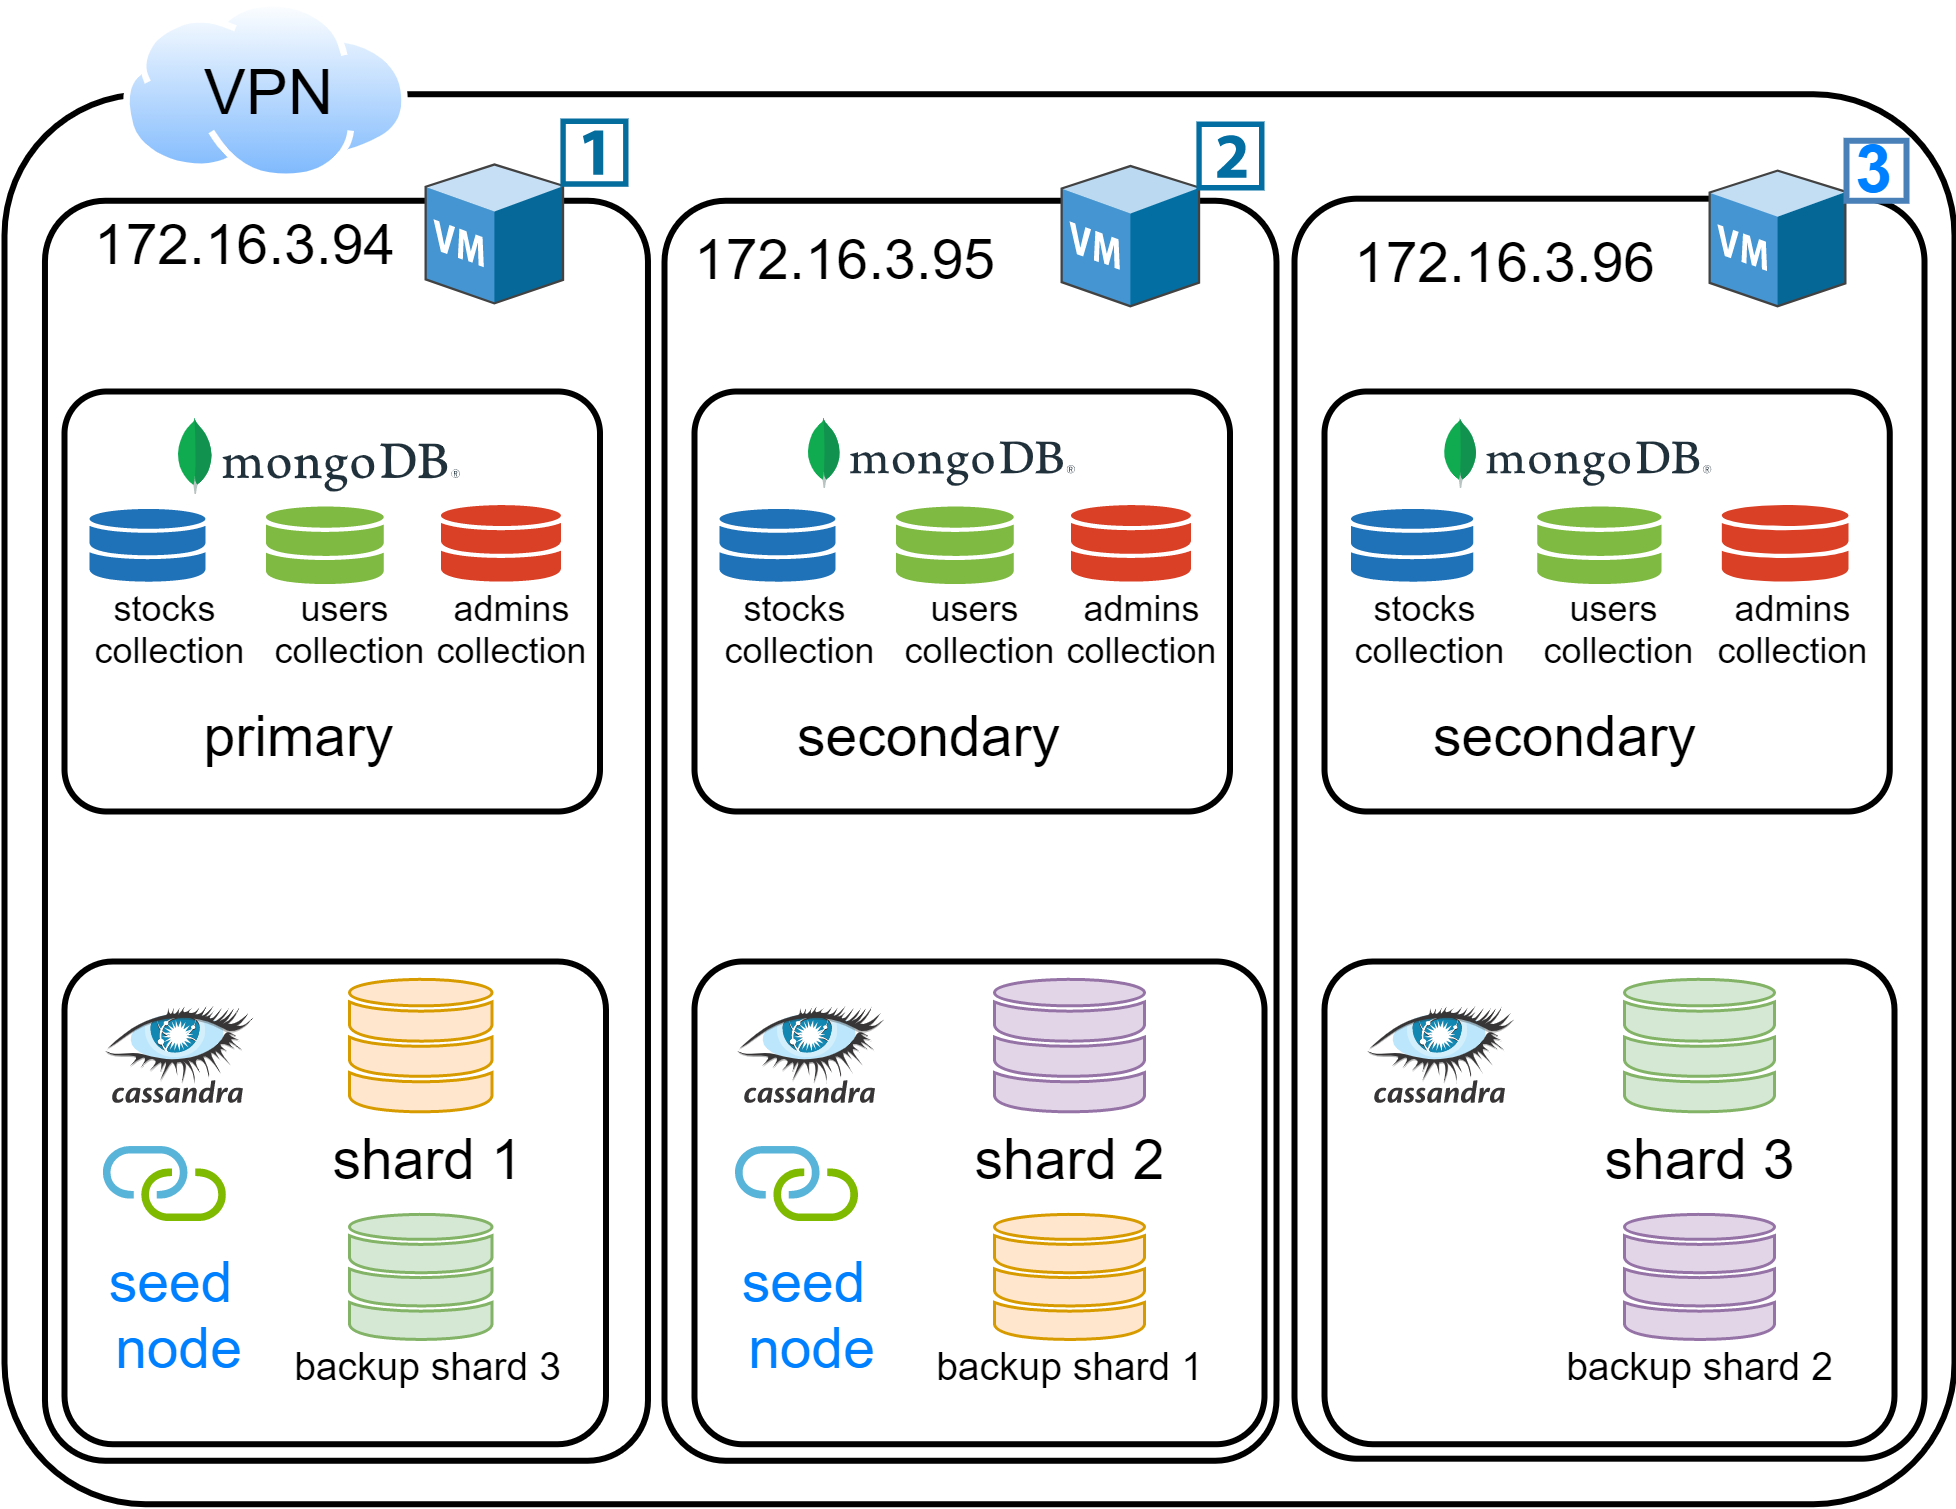
\includegraphics[scale=0.2]{img/cluster_diagram.png}\\
\section{Apache Cassandra vs MongoDB}
Cassandra and MongoDB are different database architectures but they share similar features. 
We know for sure that the usage of Cassandra can be avoided by adding a mongo Collection,
which can reproduce the behaviour of the Cassandra table for historical data. We want to explain
why in our opinion is better to store those data in Cassandra instead of Mongo, from a
performance and flexibility perspective.
\begin{itemize}
    \item 
    First of all, Cassandra has a native decentralized behaviour; we can't replicate all
    the historical data in every server, because hardware limitation, so we are forced to 
    shard data. Cassandra is specific designed for availability and partition tolerance,
    and can easy handle a node failure;
    \item 
    Cassandra can also compress data with advanced algorithms, which allow a node to store a lot
    of backup data from other nodes, increasing the availability of the service;
    \item
    Even if Mongo can store and aggregate our dataset in a decent way, the opportunity to
    create custom aggregation directly in Java language make Cassandra the best choice; this 
    allow us to perform every aggregation function that we need, and to add new ones;
    \item
    From a performance perspective, we ran the same query, on the same dataset, with the same 
    indexes structure, both in a Mongo collection and in our Cassandra keyspace; Cassandra
    always registered no latency, while mongo showed some ms of latency (4 in most cases);
    tests were performed on local storage, in the same machine,
    because remote latency performance would have been 
    somehow distorted by network swings.\\
    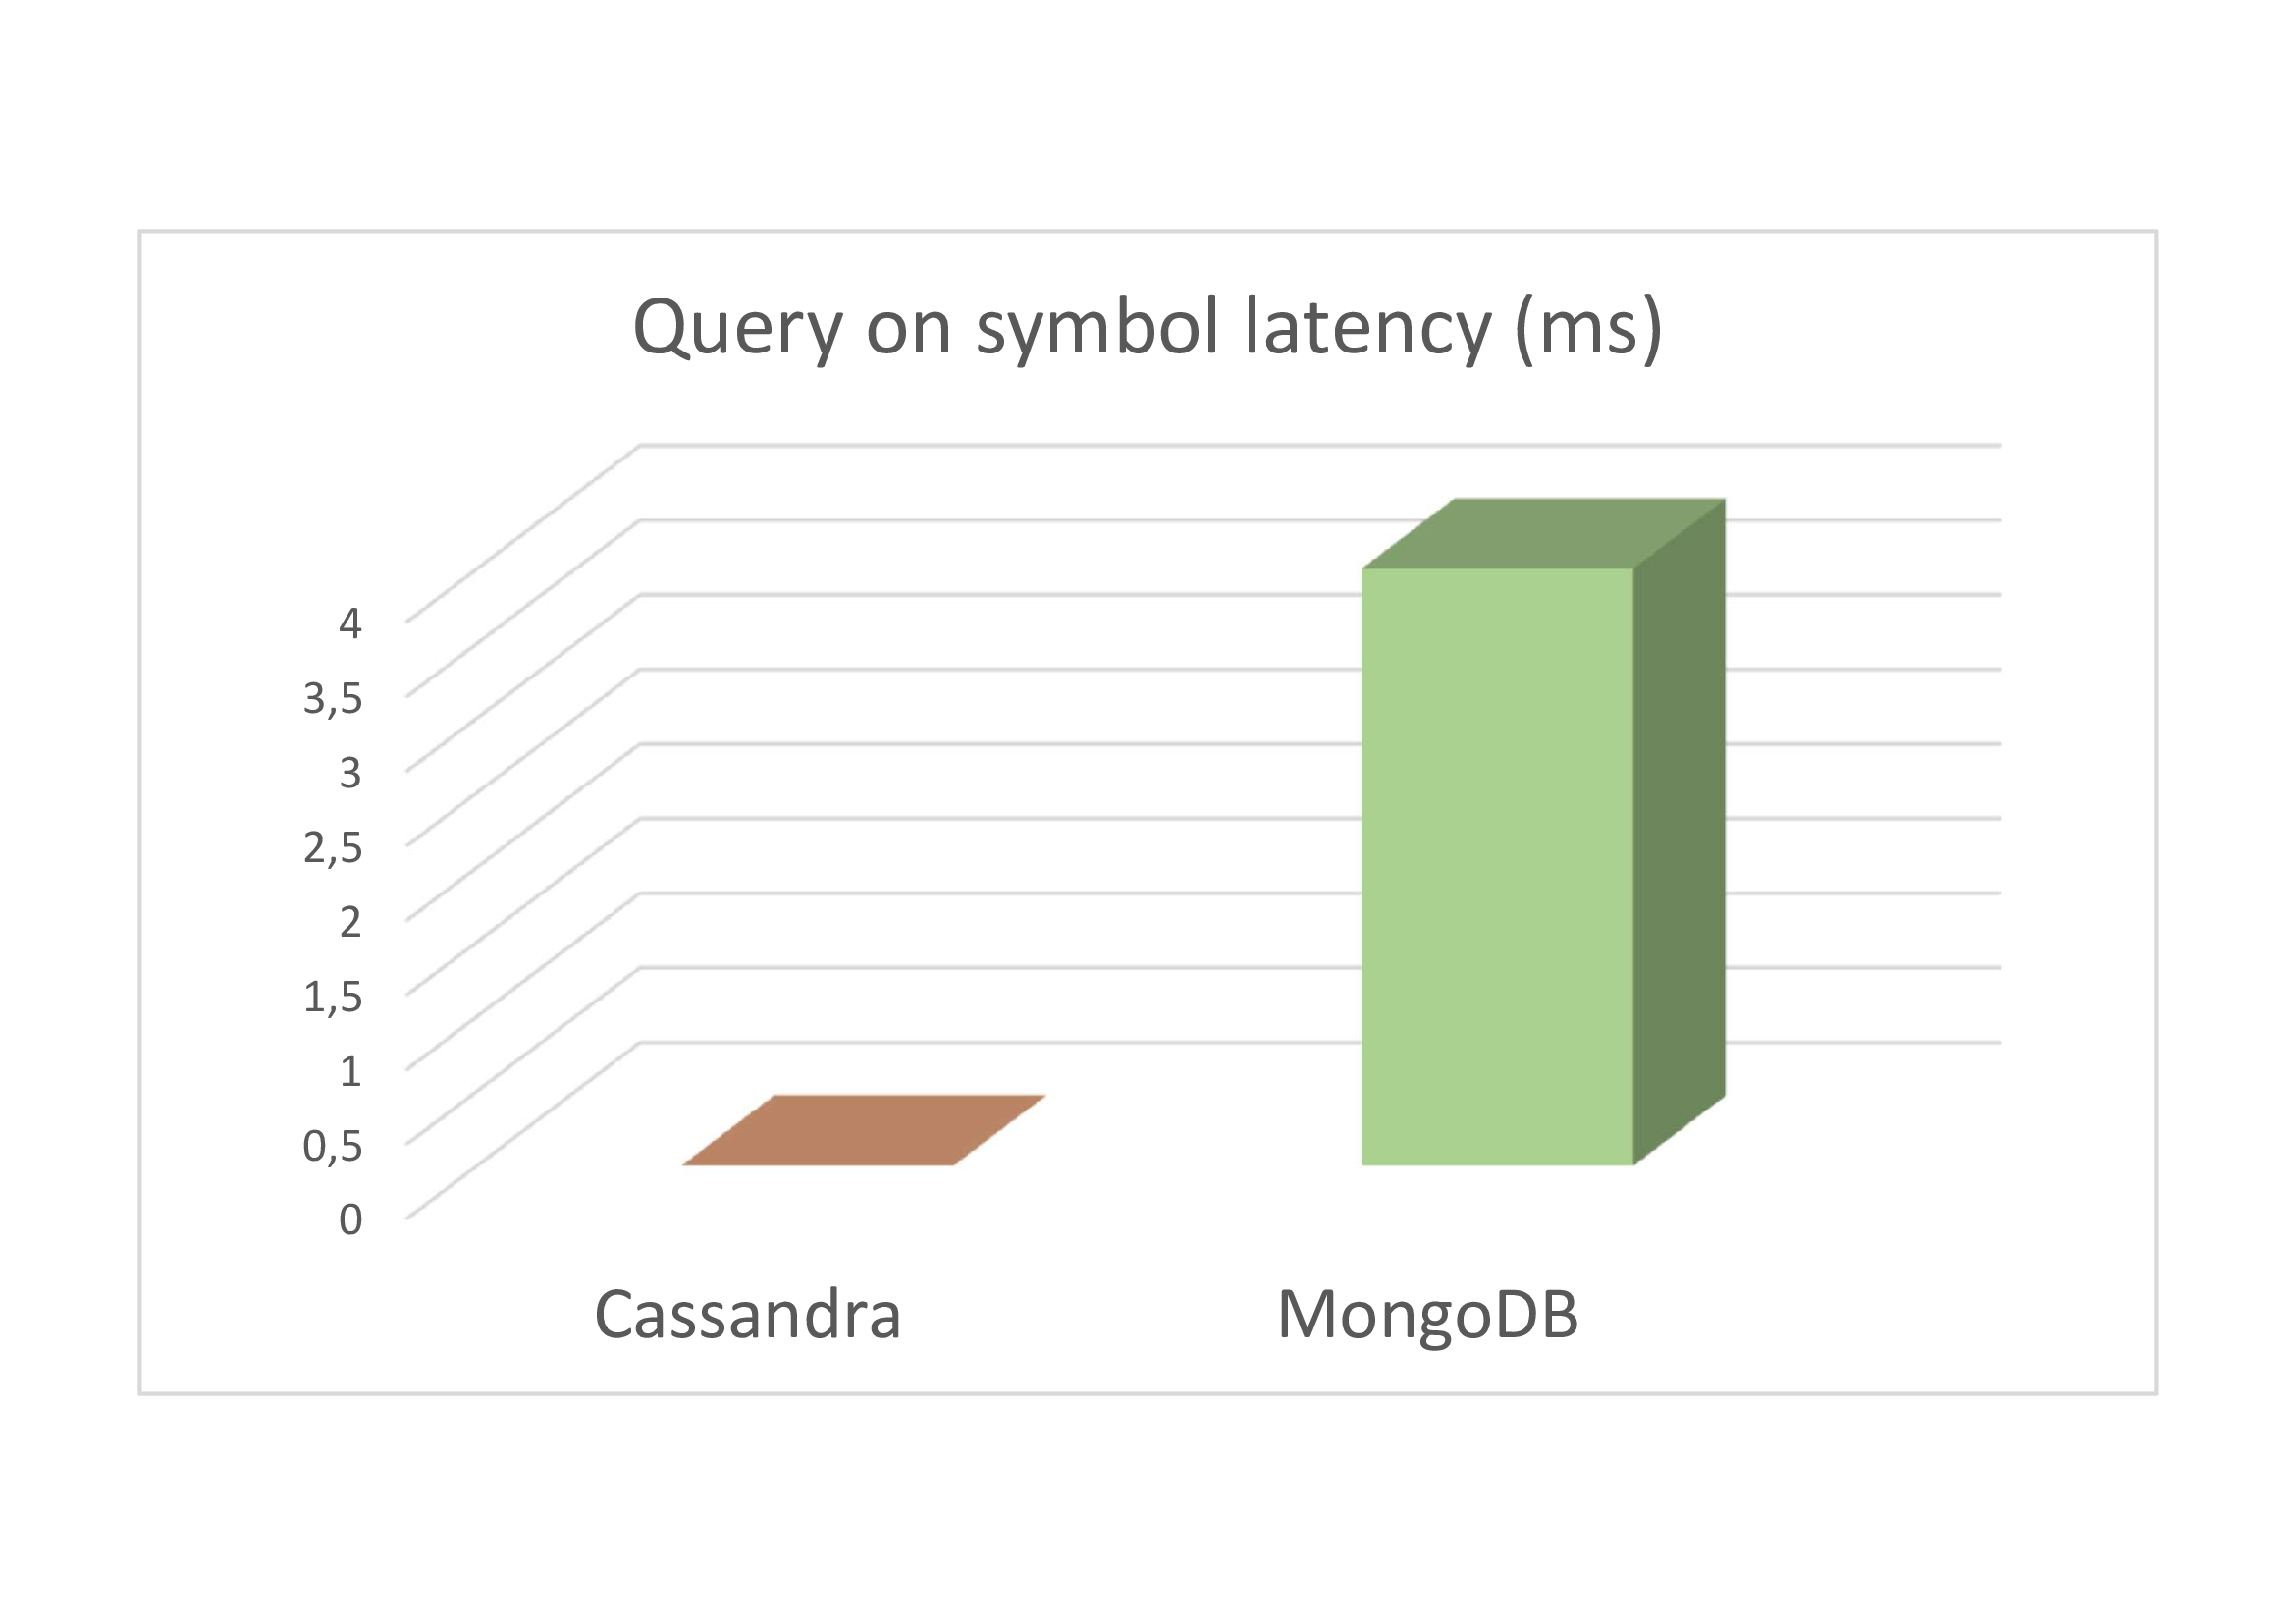
\includegraphics[scale=0.16]{img/cassandra_vs_mongoDB.png}\\

\end{itemize}

%-------------------------------------------------------------------------------
% File: software_architecture.tex
%       Part of StockSim project documentation.
%       See main.tex for further information.
%-------------------------------------------------------------------------------
\chapter{Software Architecture}
In this section the general software architecture of the application is
presented.\\
StockSim is a Java multi-module Maven application written using the IntelliJ
IDEA IDE.\\
We opted for a multi-module approach so that logically independent modules of
the applications could be kept separated and better maintained. This allowed
\begin{itemize}
    \item each of us to focus on the development of a particular module;
    \item to avoid code replication.
\end{itemize}
Furthermore, we decided to follow a feature-oriented development process and the
modularity of the project helped us code with more ease and efficiency.\\
\\
The entire codebase can be found at \url{https://github.com/rambodrahmani/stocksim}.
\section{Maven Multi-Module Structure}
The application consists of three modules: \texttt{Client}, \texttt{Server} and
\texttt{Library}.\\
The \texttt{parent} \texttt{.pom} defines the parent module Stocksim, with all
the dependencies and build settings that are common to the child modules.\\
\begin{lstlisting}[basicstyle=\footnotesize,language=Java,numbers=left,
    numberstyle=\footnotesize,numbersep=4pt,frame=single]
<?xml version="1.0" encoding="UTF-8"?>
<project xmlns="http://maven.apache.org/POM/4.0.0"
         xmlns:xsi="http://www.w3.org/2001/XMLSchema-instance"
         xsi:schemaLocation="http://maven.apache.org/POM/4.0.0 http://maven.apache.org/xsd/maven-4.0.0.xsd">
    <modelVersion>4.0.0</modelVersion>
    <groupId>it.unipi.lsmsdb.workgroup4</groupId>
    <artifactId>Stocksim</artifactId>
    <packaging>pom</packaging>
    <version>1.0</version>

    <!-- child modules -->
    <modules>
        <module>Client</module>
        <module>Server</module>
        <module>Library</module>
    </modules>

    [...]
\end{lstlisting}
Each child module has its own \texttt{.pom} file, necessary for the building
process and for keeping track of all the required dependencies.\\
\begin{lstlisting}[basicstyle=\footnotesize,language=Java,numbers=left,
    numberstyle=\footnotesize,numbersep=4pt,frame=single]
<?xml version="1.0" encoding="UTF-8"?>
<project xmlns="http://maven.apache.org/POM/4.0.0"
         xmlns:xsi="http://www.w3.org/2001/XMLSchema-instance"
         xsi:schemaLocation="http://maven.apache.org/POM/4.0.0 http://maven.apache.org/xsd/maven-4.0.0.xsd">
    <parent>
        <artifactId>Stocksim</artifactId>
        <groupId>it.unipi.lsmsdb.workgroup4</groupId>
        <version>1.0</version>
    </parent>

    <!-- child module -->
    <modelVersion>4.0.0</modelVersion>
    <artifactId>Server</artifactId>
    <packaging>jar</packaging>

    <!-- dependencies -->
    <dependencies>
        <dependency>
            <groupId>it.unipi.lsmsdb.workgroup4</groupId>
            <artifactId>Library</artifactId>
            <version>1.0-SNAPSHOT</version>
            <scope>compile</scope>
        </dependency>
        <dependency>
            <groupId>it.unipi.lsmsdb.workgroup4</groupId>
            <artifactId>Library</artifactId>
            <version>1.0</version>
            <scope>compile</scope>
        </dependency>
    </dependencies>

    [...]
\end{lstlisting}
For the full content of the \texttt{.pom} files please refer to Appendix A.
\subsection{Library}
The \texttt{Library} module, contains the database APIs both for MongoDB and
Apache Cassandra, together with the YahooFinance API and some utility functions.
The \texttt{Library} module was created in order to avoid code replication. The
\texttt{Client} and \texttt{Server} module relay on the APIs implemented in this
module.\\
It has the following structure:
\vspace{0.2cm}
\dirtree{%
.1 LIBRARY.
.2 src.
.3 main.
.4 java.
.5 it.unipi.lsmsdb.stocksim.lib.
.6 database.
.7 cassandra.
.7 mongoDB.
.6 util.
.6 yfinance.
}
\vspace{0.2cm}
\noindent The \texttt{database} package contains the two APIs we wrote for the
interaction with Apache Cassandra and MongoDB.\\
The \texttt{yfinance} package contains the API used to retrieve data from
Yahoo Finance. After trying some of the offered APIs, we decided to implement
our own from scratch.\\
The \texttt{util} package contains some utilities functions, such as the ones 
used to set the log level both for Apache Cassandra and MongoDB, and our custom
argument parser derived from \texttt{Apache Commons CLI} used to parse command
line arguments for both StockSim Server and StockSim Client.
\begin{figure}[H]
\begin{subfigure}{.3\textwidth}
  \hspace{-3.0cm}
  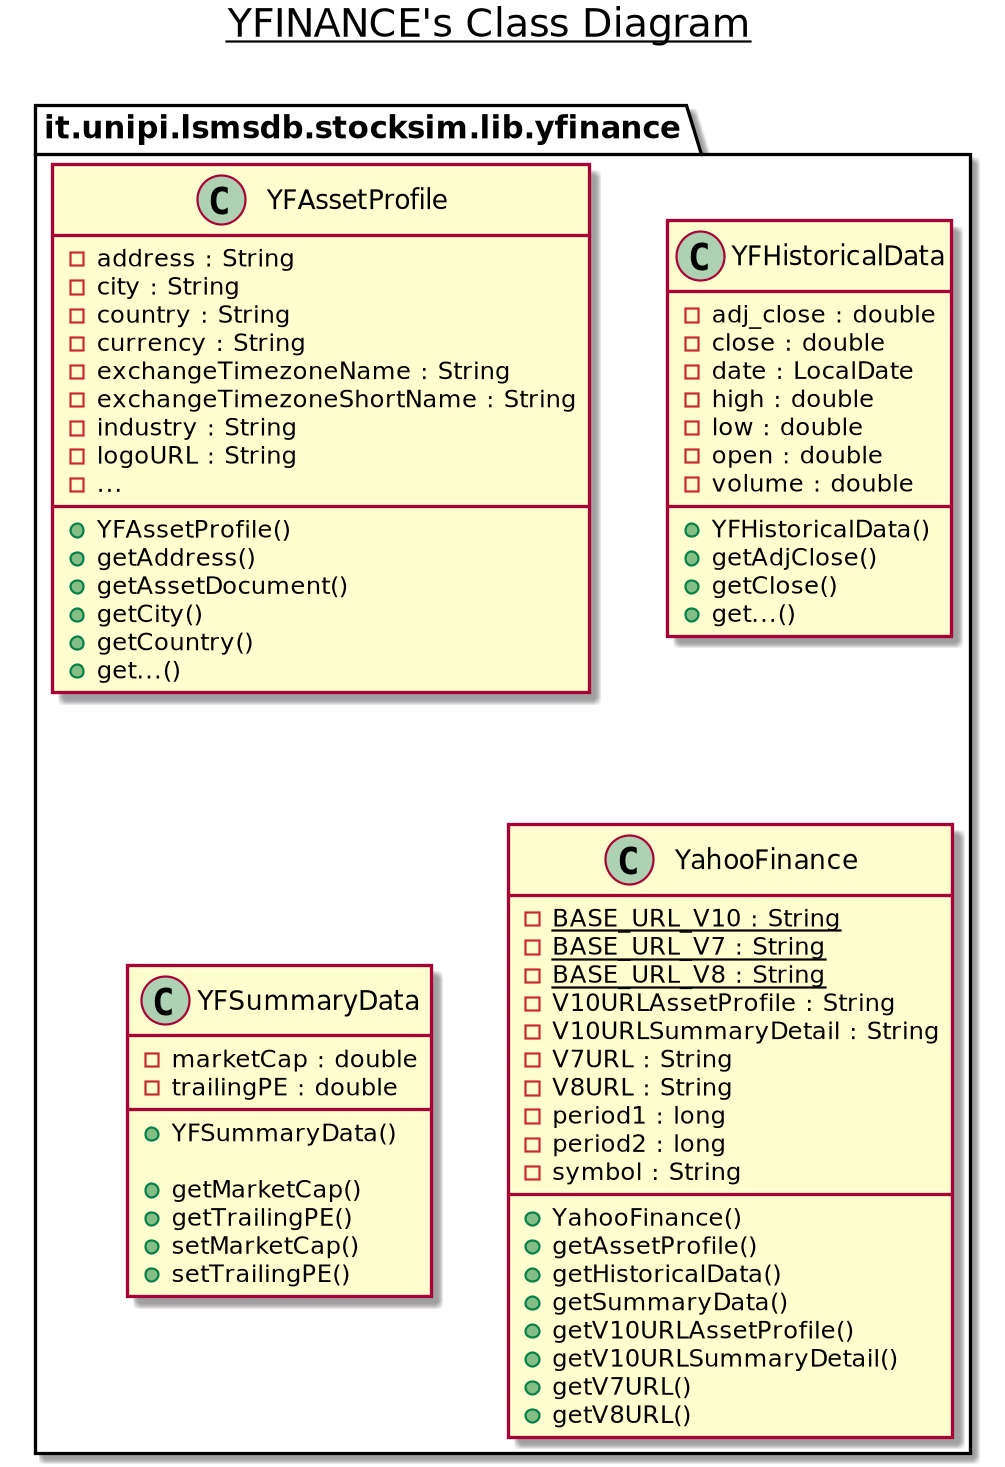
\includegraphics[scale=0.16]{plantuml/library/yfinance.png}
\end{subfigure}%
\hspace{-1.0cm}
\begin{subfigure}{.3\textwidth}
  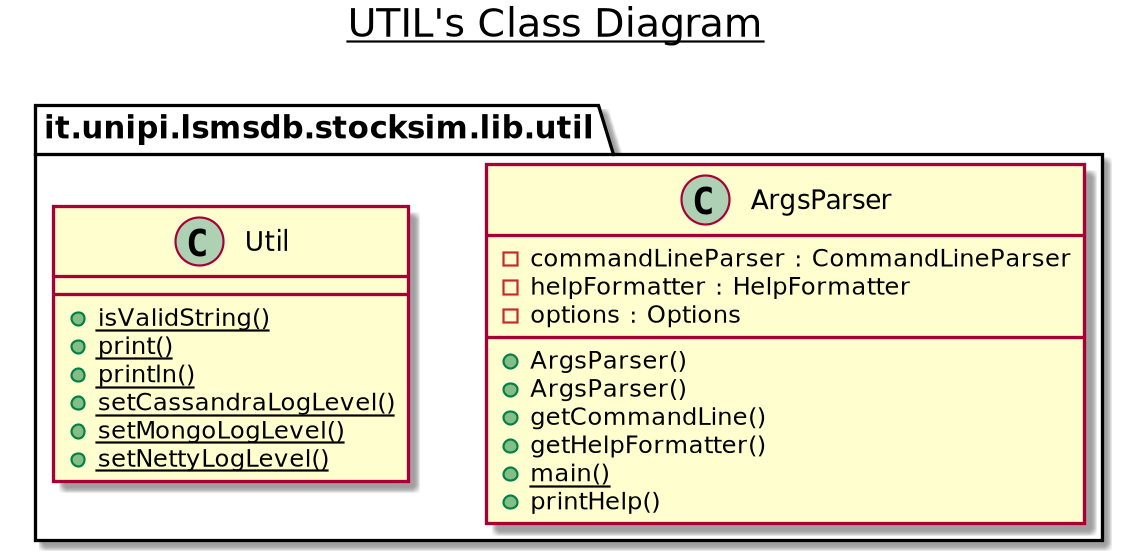
\includegraphics[scale=0.2]{plantuml/library/util.png}
\end{subfigure}
\hspace{4.0cm}
\begin{subfigure}{.3\textwidth}
  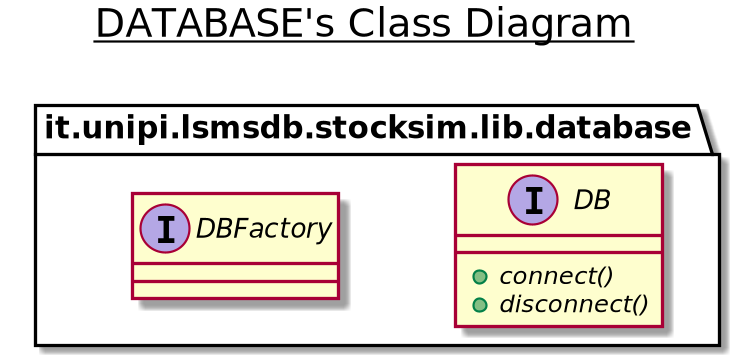
\includegraphics[scale=0.2]{plantuml/library/database.png}
\end{subfigure}
\end{figure}
\begin{figure}[H]
\begin{subfigure}{.5\textwidth}
  \hspace{-3.0cm}
  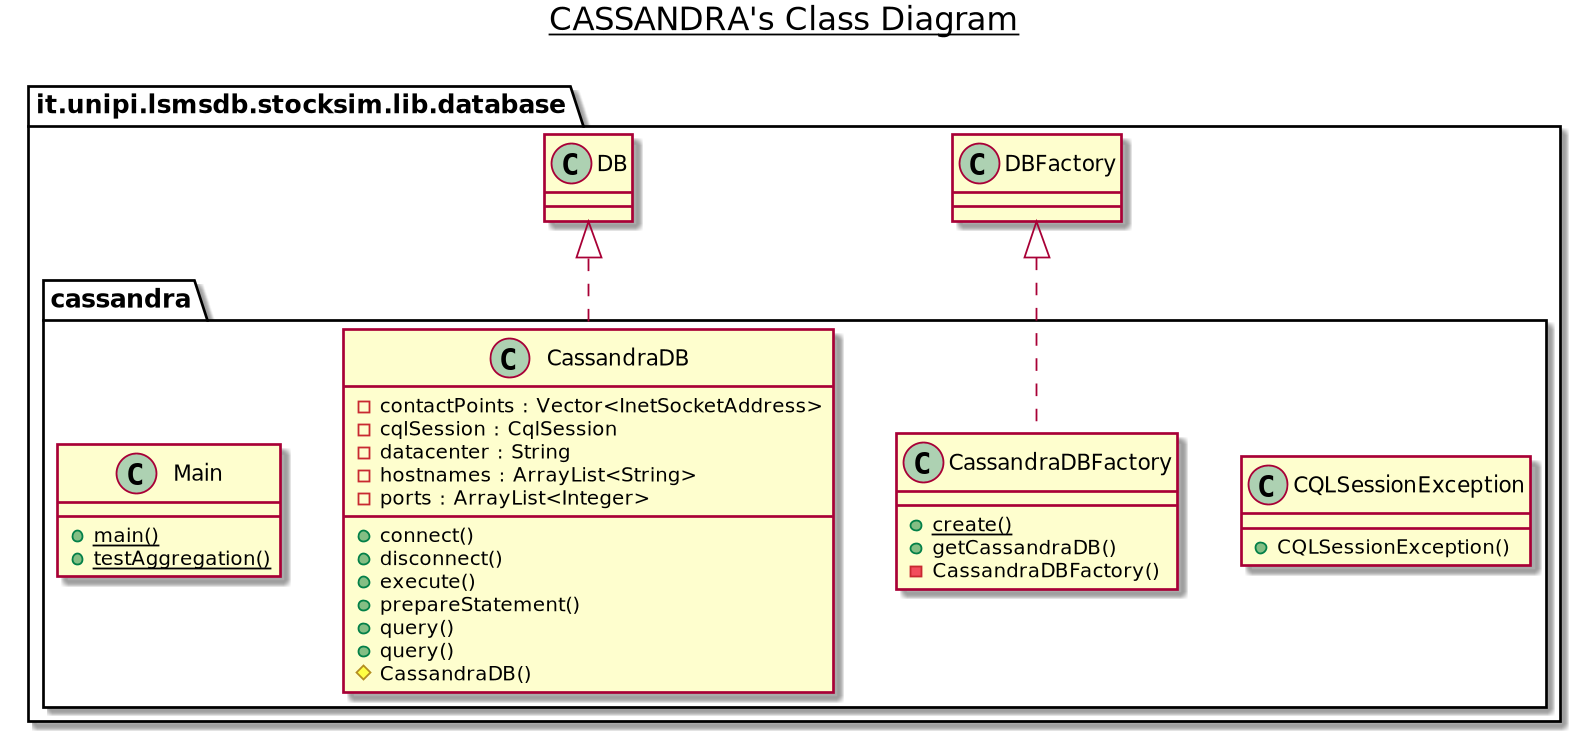
\includegraphics[scale=0.2]{plantuml/library/cassandra.png}
\end{subfigure}%
\hspace{1.0cm}
\begin{subfigure}{.5\textwidth}
  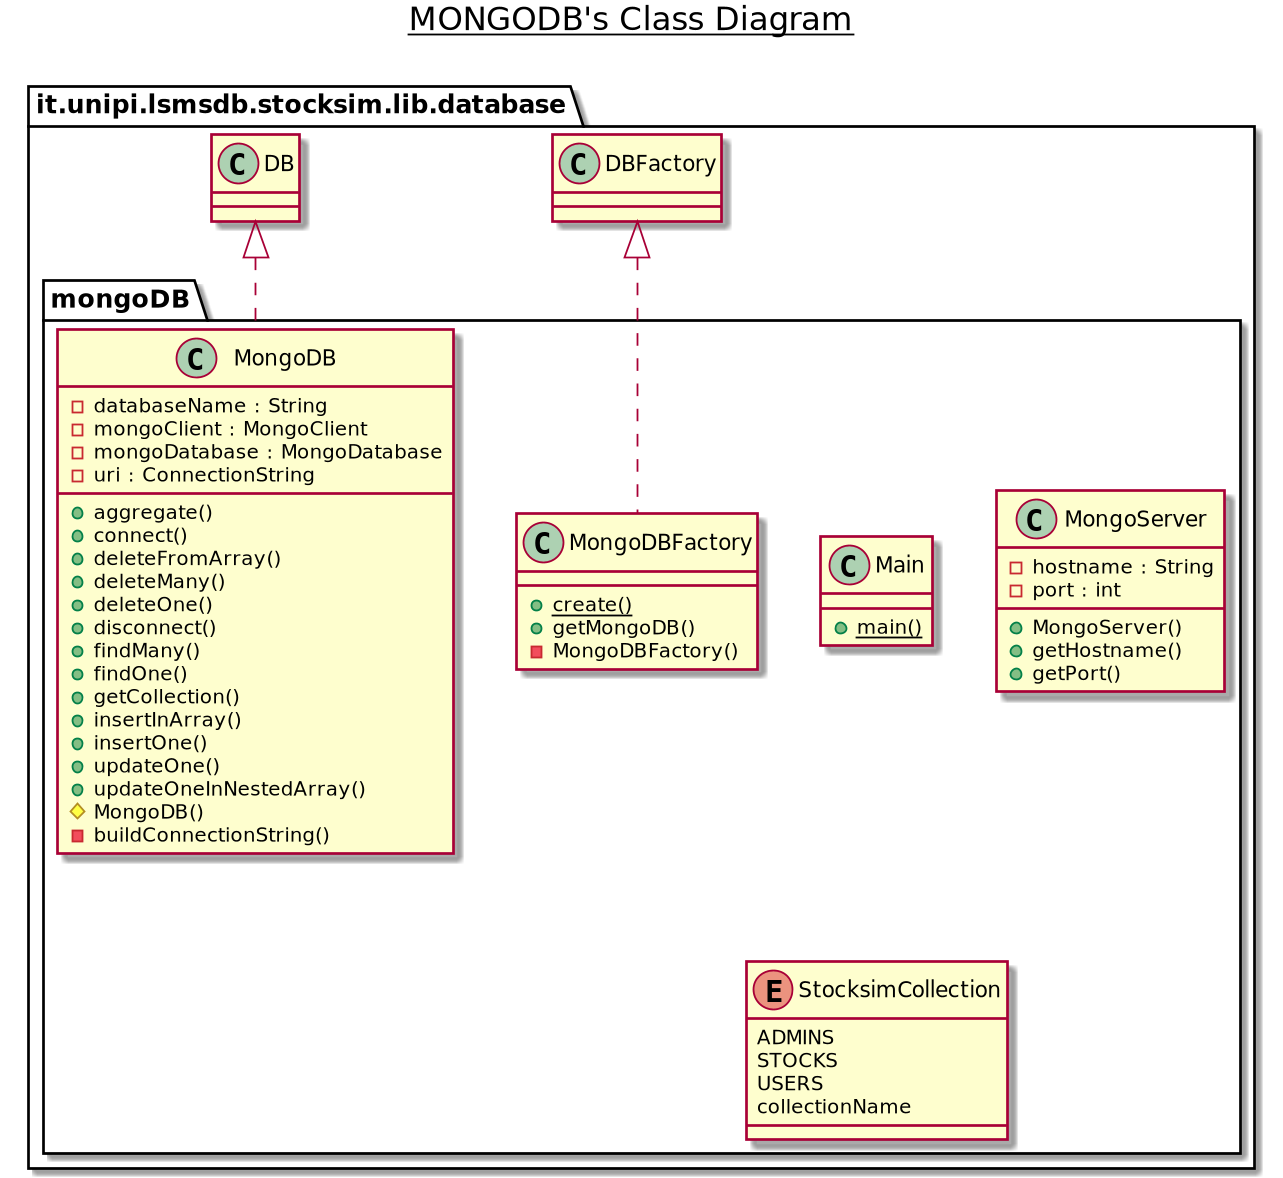
\includegraphics[scale=0.2]{plantuml/library/mongoDB.png}
\end{subfigure}
\caption{Library Module UML sample Diagrams}
\end{figure}
\subsection{Client}
The Client module contains the StockSim Client implementation. This program is
intended to be distributed to end users.\\
It has the following structure:
\vspace{0.2cm}
\dirtree{%
.1 CLIENT.
.2 src.
.3 main.
.4 java.
.5 it.unipi.lsmsdb.stocksim.client.
.6 admin.
.6 app.
.6 charting.
.6 database.
.6 user.
.3 resources.
}
\vspace{0.2cm}
\noindent The \texttt{app} directory contains the \texttt{Client.java} class
with the entry point for the application.\\
Since the StockSim Client program was thought to be executed in two different
running modes (namely \texttt{admin} or \texttt{user} mode), the \texttt{admin}
and \texttt{user} packages contain the implementation of the functionalities
available to the user in these two different running modes.
The \texttt{database} directory contains the classes necessary for the
connection management and the interaction with MongoDB and Apache Cassandra.
Also here you can find classes intended for storing the retrieved data.\\
The \texttt{charting} directory contains an API for the \texttt{JFreeChart}
library, used by the Client to create charts of various types.
\begin{figure}[H]
	\begin{center}
        \hspace*{-3.3cm}
		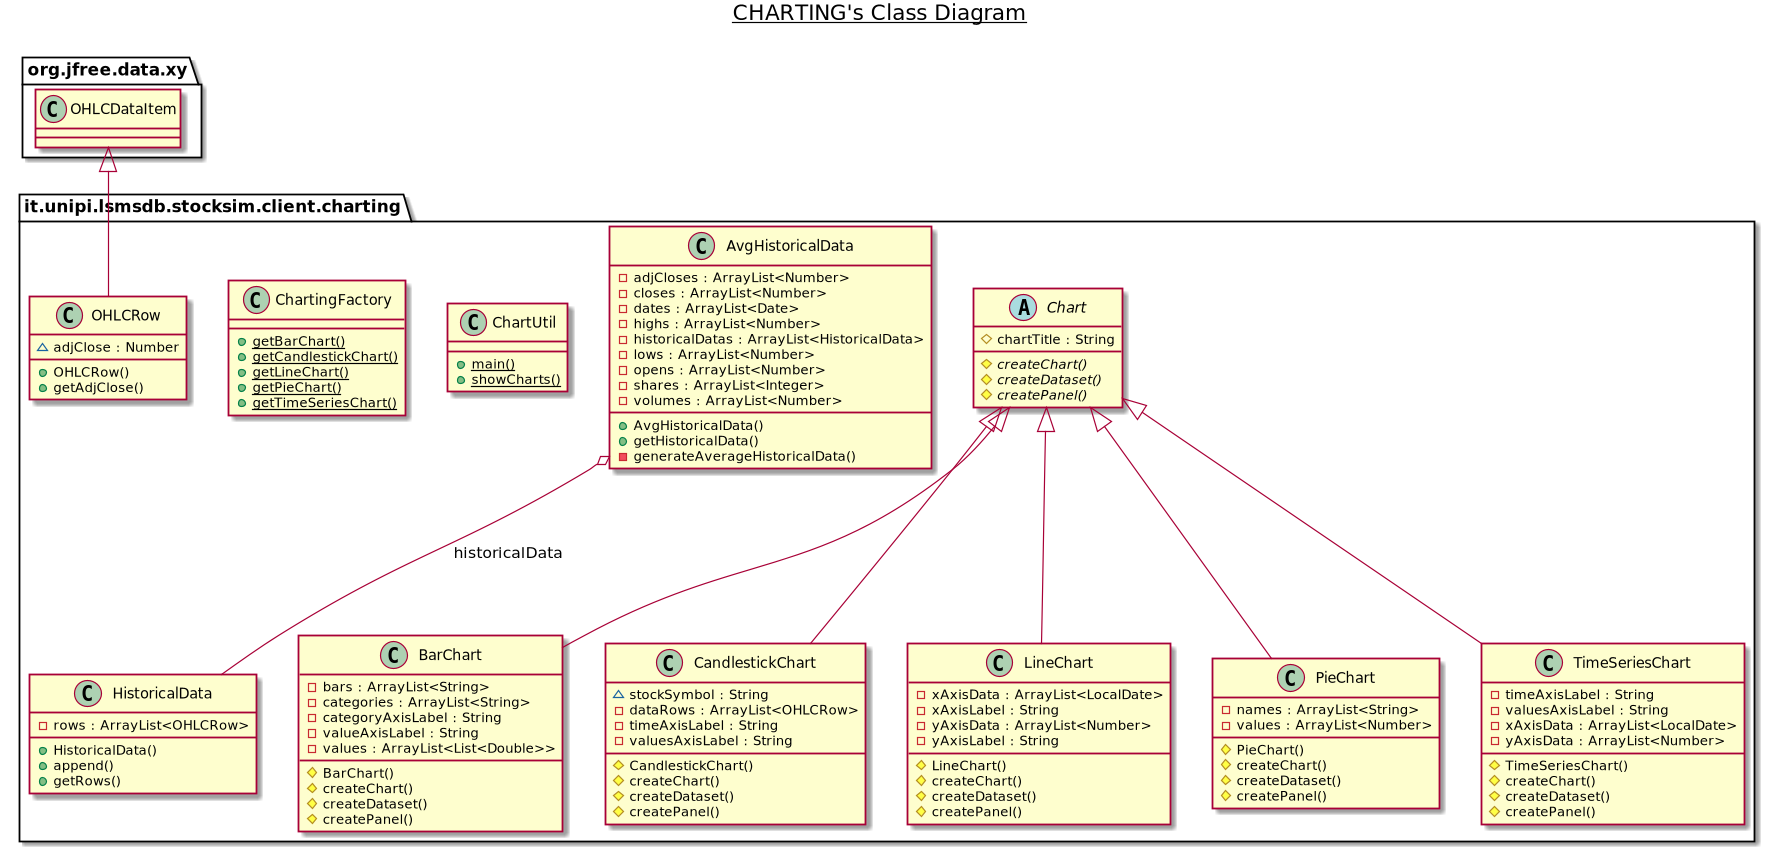
\includegraphics[scale=0.337]{plantuml/client/charting.png}
		\caption{Client charting package UML Diagram as sample}
	\end{center}
\end{figure}
\subsection{Server}
The Server module represents the StockSim Server program which takes care of
keeping the data updated and consistent.\\
It is not supposed to be distributed: it should be always running in order to be
able to retrieve the historical data prices relative to the latest trading
session.\\
The Server module has the following structure:
\vspace{0.2cm}
\dirtree{%
.1 SERVER.
.2 src.
.3 main.
.4 java.
.5 it.unipi.lsmsdb.stocksim.server.
.6 app.
.7 Server.java.
.7 ServerUtil.java.
.6 database.
.7 CassandraQueryBuilder.java.
.7 DBManager.java.
}
\vspace{0.2cm}
\noindent The \texttt{app} package contains the class with the entry point for
the application.\\
The \texttt{database} package contains the classes necessary for the interaction
with the databases.
\begin{figure}[H]
\begin{subfigure}{.5\textwidth}
  \hspace{-2.0cm}
  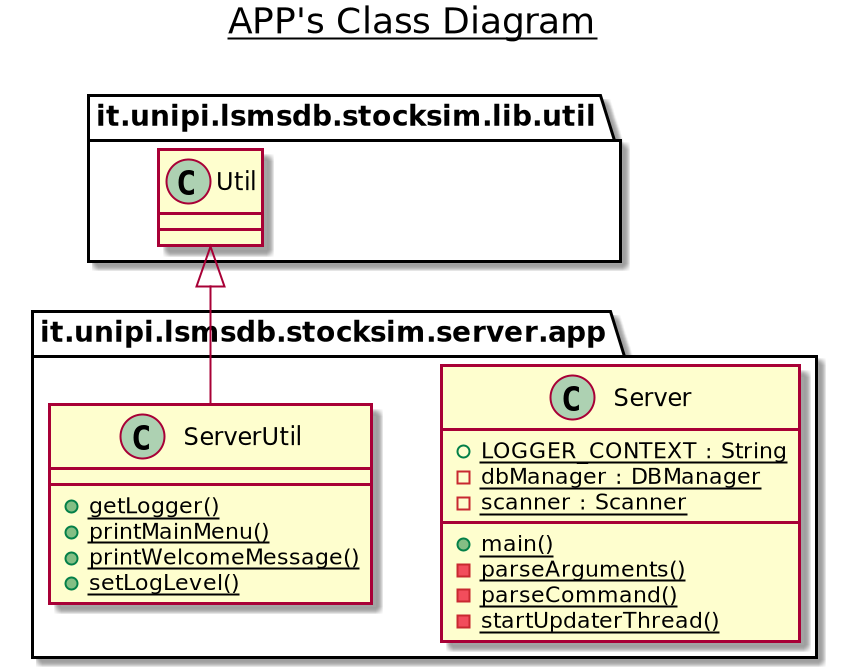
\includegraphics[scale=0.2]{plantuml/server/app.png}
\end{subfigure}%
\hspace{-2.0cm}
\begin{subfigure}{.5\textwidth}
  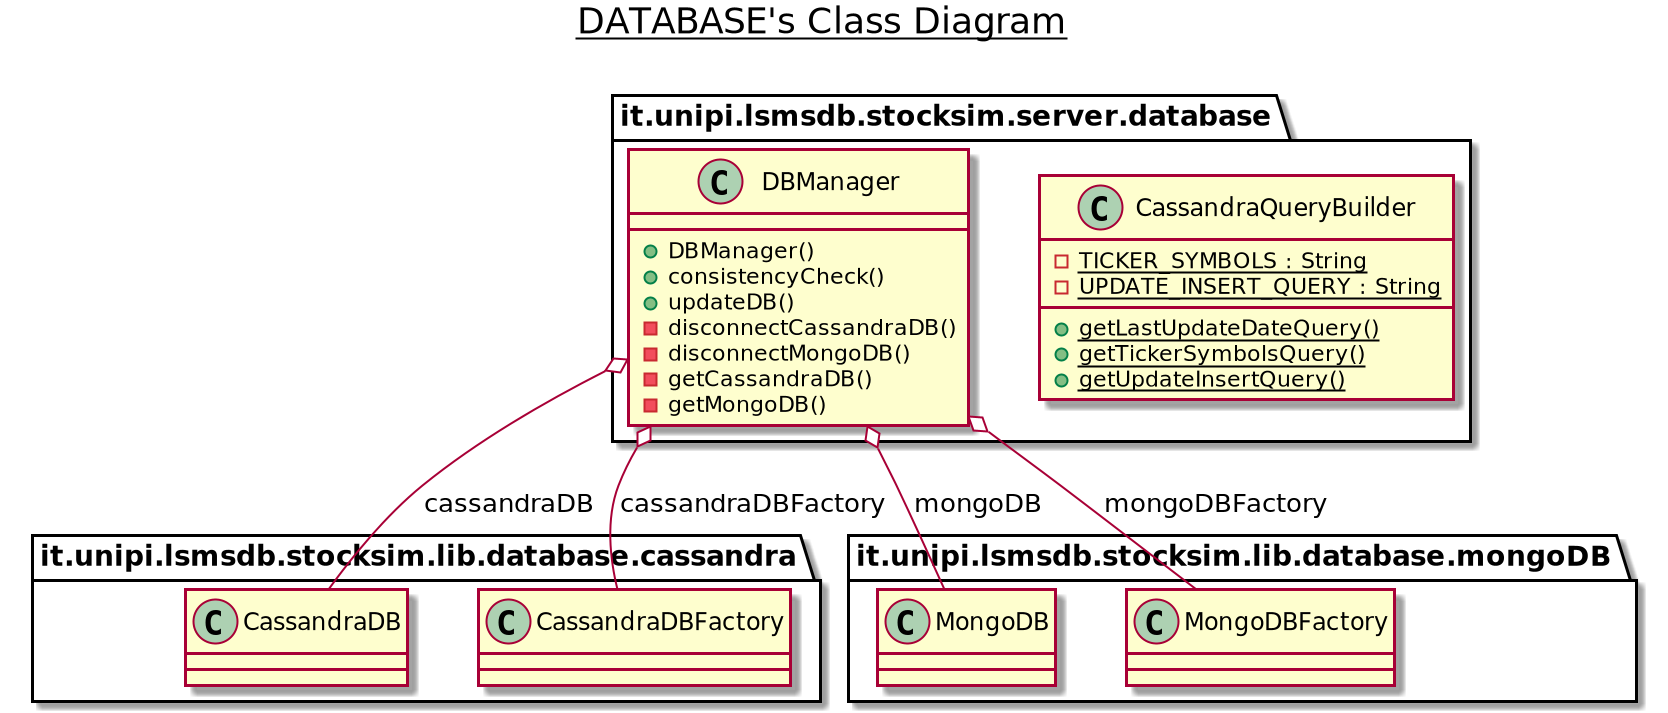
\includegraphics[scale=0.2]{plantuml/server/database.png}
\end{subfigure}
\caption{Server Module UML sample Diagrams}
\end{figure}
\section{Apache Maven Assembly Plugin}
The Assembly Plugin for Maven enables developers to combine project output into 
a single distributable archive that also contains dependencies, modules, site 
documentation, and other files.
For every module an independent .jar file can be generated  which allows to run that module \textit{standalone}, without any dependency issue.

%-------------------------------------------------------------------------------
% File: conclusions.tex
%       Part of StockSim project documentation.
%       See main.tex for further information.
%-------------------------------------------------------------------------------
\chapter{Conclusions}


\afterpage{\blankpage}

%-------------------------------------------------------------------------------
% File: appendices.tex
%       Part of StockSim project documentation.
%       See main.tex for further information.
%-------------------------------------------------------------------------------
\chapter{Appendices}

\chapter*{Appendix A}
%TODO reduce spacing before chapter title so that first pom is not broken in 3 pages but only in 2.

\lstinputlisting[basicstyle=\footnotesize,language=XML,numbers=left,
numberstyle=\footnotesize,numbersep=8pt,frame=single]{pom_files/parent_pom.xml}

\lstinputlisting[basicstyle=\footnotesize,language=XML,numbers=left,
numberstyle=\footnotesize,numbersep=8pt,frame=single]{pom_files/client_pom.xml}

\lstinputlisting[basicstyle=\footnotesize,language=XML,numbers=left,
numberstyle=\footnotesize,numbersep=8pt,frame=single]{pom_files/server_pom.xml}

\lstinputlisting[basicstyle=\footnotesize,language=XML,numbers=left,
numberstyle=\footnotesize,numbersep=8pt,frame=single]{pom_files/library_pom.xml}

%-------------------------------------------------------------------------------
% Part I: User Manual
%-------------------------------------------------------------------------------
\part{User Manual}
%-------------------------------------------------------------------------------
% File: user_manual_CH1.tex
%       Part of StockSim project documentation.
%       See main.tex for further information.
%-------------------------------------------------------------------------------
\chapter{StockSim Server Manual}
For an application dealing with the stock market, it is essential to 
always provide up-to-date, consistent and reliable data. This is the purpose of 
the \textbf{StockSim Server} program. It is not intended to be distributed to 
end users. It is thought to be running 24/7.\\
\\
The StockSim Server has two different startup modes: the first one
\begin{lstlisting}[basicstyle=\footnotesize,language=bash,numbers=left,
numberstyle=\footnotesize,numbersep=8pt,frame=single]
$ java -jar Server.jar

Welcome to the StockSim Server.

DATA CONSISTENCY CHECK SUCCESS. PROCEEDING WITH UPDATE.

Updating historical data for: IRBT.
Last update date: 2020-12-30.
Days since last update: 2.
Historical data updated for IRBT. Moving on.

...

Updating historical data for: EWU.
Last update date: 2020-12-28.
Days since last update: 4.
Historical data updated for EWU. Moving on.

...


\end{lstlisting}
which executes the \texttt{historical data update} procedure right after
startup. Whereas, the second startup mode can be triggered using the
\texttt{--no-update} command line argument:
\begin{lstlisting}[basicstyle=\footnotesize,language=bash,numbers=left,
numberstyle=\footnotesize,numbersep=8pt,frame=single]
$ java -jar Server.jar --no-update

Welcome to the StockSim Server.

Available Commands:
status       check databases status.                 
update       update databases historical data.       
quit         quit Stocksim server.                   
> 
[UPDATER THREAD] Current New York time: 2021-01-02T06:29-[America/New_York]
[UPDATER THREAD] Going to sleep for 14 hours before next update.
> update

DATA CONSISTENCY CHECK SUCCESS. PROCEEDING WITH UPDATE.

Updating historical data for: IRBT.
Last update date: 2020-12-30.
Days since last update: 2.
Historical data updated for IRBT. Moving on.

...

Updating historical data for: EWU.
Last update date: 2020-12-28.
Days since last update: 4.
Historical data updated for EWU. Moving on.

...

\end{lstlisting}
in this mode, no update is executed right after startup, the main menu is shown
and the user can decide the action to be performed.\\
\\
In the previously shown examples, we should pay attention to the following
\begin{itemize}
    \item \texttt{DATA CONSISTENCY CHECK SUCCESS. PROCEEDING WITH UPDATE.}
    \item \texttt{the sotcksim server automatically detects the last update
    date, the number of days since the last update and fetches the required
    data using Yahoo Finance for EACH and EVERY ticker symbol.}
    \item \texttt{Historical Data Update logs.}
    \item \texttt{[UPDATER THREAD]}
\end{itemize}

%-------------------------------------------------------------------------------
% File: user_manual_CH2.tex
%       Part of StockSim project documentation.
%       See main.tex for further information.
%-------------------------------------------------------------------------------
\chapter{StockSim Client Manual}
The StockSim Client has two different running modes: the first one
\begin{lstlisting}[basicstyle=\footnotesize\ttfamily,language={},numbers=left,keepspaces=true,tabsize=4,
numberstyle=\footnotesize,numbersep=8pt,frame=single]
Welcome to the StockSim Client.

*** [RUNNING IN USER MODE] ***

Available Commands:
register		create a new user account.              
login			login to your user account.             
quit			quit StockSim client. 
\end{lstlisting}
is the \texttt{user mode}. Whereas, the second running mode can be triggered 
using the \texttt{--admin} command line argument:
\begin{lstlisting}[basicstyle=\footnotesize\ttfamily,language={},numbers=left,keepspaces=true,tabsize=4,
numberstyle=\footnotesize,numbersep=8pt,frame=single]
$ java -jar Client.jar --admin

Welcome to the StockSim Client.

*** [RUNNING IN ADMIN MODE] ***

Available Commands:
login		login to your admin account.            
quit		quit StockSim client.
\end{lstlisting}
and is the \texttt{admin mode}. Although they might look like the same, the 
available menu actions differ once the user/admin login has been executed.

\section{StockSim Client User Mode}
Upon launching the application in \textit{user} mode, the user is presented with three options: \textit{register}, \textit{login} and \textit{quit}.\\
After selecting \textit{register}, the user is asked to enter their info, such as name, surname, email, username and password:
\begin{lstlisting}[basicstyle=\footnotesize\ttfamily,language={},numbers=left,keepspaces=true,tabsize=4,
numberstyle=\footnotesize,numbersep=8pt,frame=single]
> register
Name: John
Surname: Smith
E-Mail: jsmith@example.com
Username [login]: jsmith
Password [login]: hunter2
User sign up executed correctly. You can now login.
\end{lstlisting}

Once the user is registered and logged in, the application offers several options:

\begin{lstlisting}[basicstyle=\footnotesize\ttfamily,language={},numbers=left,keepspaces=true,tabsize=4,
numberstyle=\footnotesize,numbersep=8pt,frame=single]
> login
Username: jsmith
Password: hunter2
User login executed correctly.
Welcome John Smith.

[jsmith] Available Commands:
search-stock			search for a stock ticker.              
view-stock				view historical data for a stock ticker.
create-portfolio		create a new stock portfolio.           
list-portfolios			list user stock portfolios.             
view-portfolio			view user stock portfolio info.         
simulate-portfolio		simulate user stock portfolio.          
delete-portfolio		delete user stock portfolio.            
logout					logout from current user account.       
quit					quit StockSim client.   
\end{lstlisting}

\subsection{Search stock}
The \texttt{search-stock} option allows the user to search for a specific stock in the database. The search can be done by \textbf{symbol}, by \textbf{sector} or by \textbf{country}.\\

\begin{lstlisting}[basicstyle=\footnotesize\ttfamily,language={},numbers=left,keepspaces=true,tabsize=4,
numberstyle=\footnotesize,numbersep=8pt,frame=single]
> search-stock
[jsmith] Available Search Commands:
symbol-search			search for a stock ticker using its ticker.
sector-search			search for a stock ticker using the sector.
country-search			search for a stock ticker using the country.
\end{lstlisting}
A search by symbol prompts the user for the symbol of the stock to be searched and returns all the information available in the database about that stock.
\begin{lstlisting}[basicstyle=\footnotesize\ttfamily,language={},numbers=left,keepspaces=true,tabsize=4,
numberstyle=\footnotesize,numbersep=8pt,frame=single]
> symbol-search
Ticker Symbol: TSLA
Short Name: Tesla, Inc.
Long Name: Tesla, Inc.
Symbol: TSLA
Quote type: EQUITY
Market capitalization: 8.00041992192E11
PE ratio: 1265.3346
Market: us_market
Exchange timezone short name: EST
Exchange timezone name: America/New_York
Sector: Consumer Cyclical
Industry: Auto Manufacturers
Currency: USD
Location:  3500 Deer Creek Road Palo Alto CA United States
650-681-5000
Logo URL: https://logo.clearbit.com/tesla.com
Website: http://www.tesla.com
Long business summary:
Tesla, Inc. designs, develops, manufactures, leases, and sells electric
vehicles, and energy [...]

\end{lstlisting}

A search by sector opens a two bar charts showing aggregated data for all sectors (one for total market capitalizaion and the other for average trailing P/E) and prompts the user for the sector they are interested in.
Once the desired sector is entered, a list with all related symbols is returned.

\hfill \break
{\centering
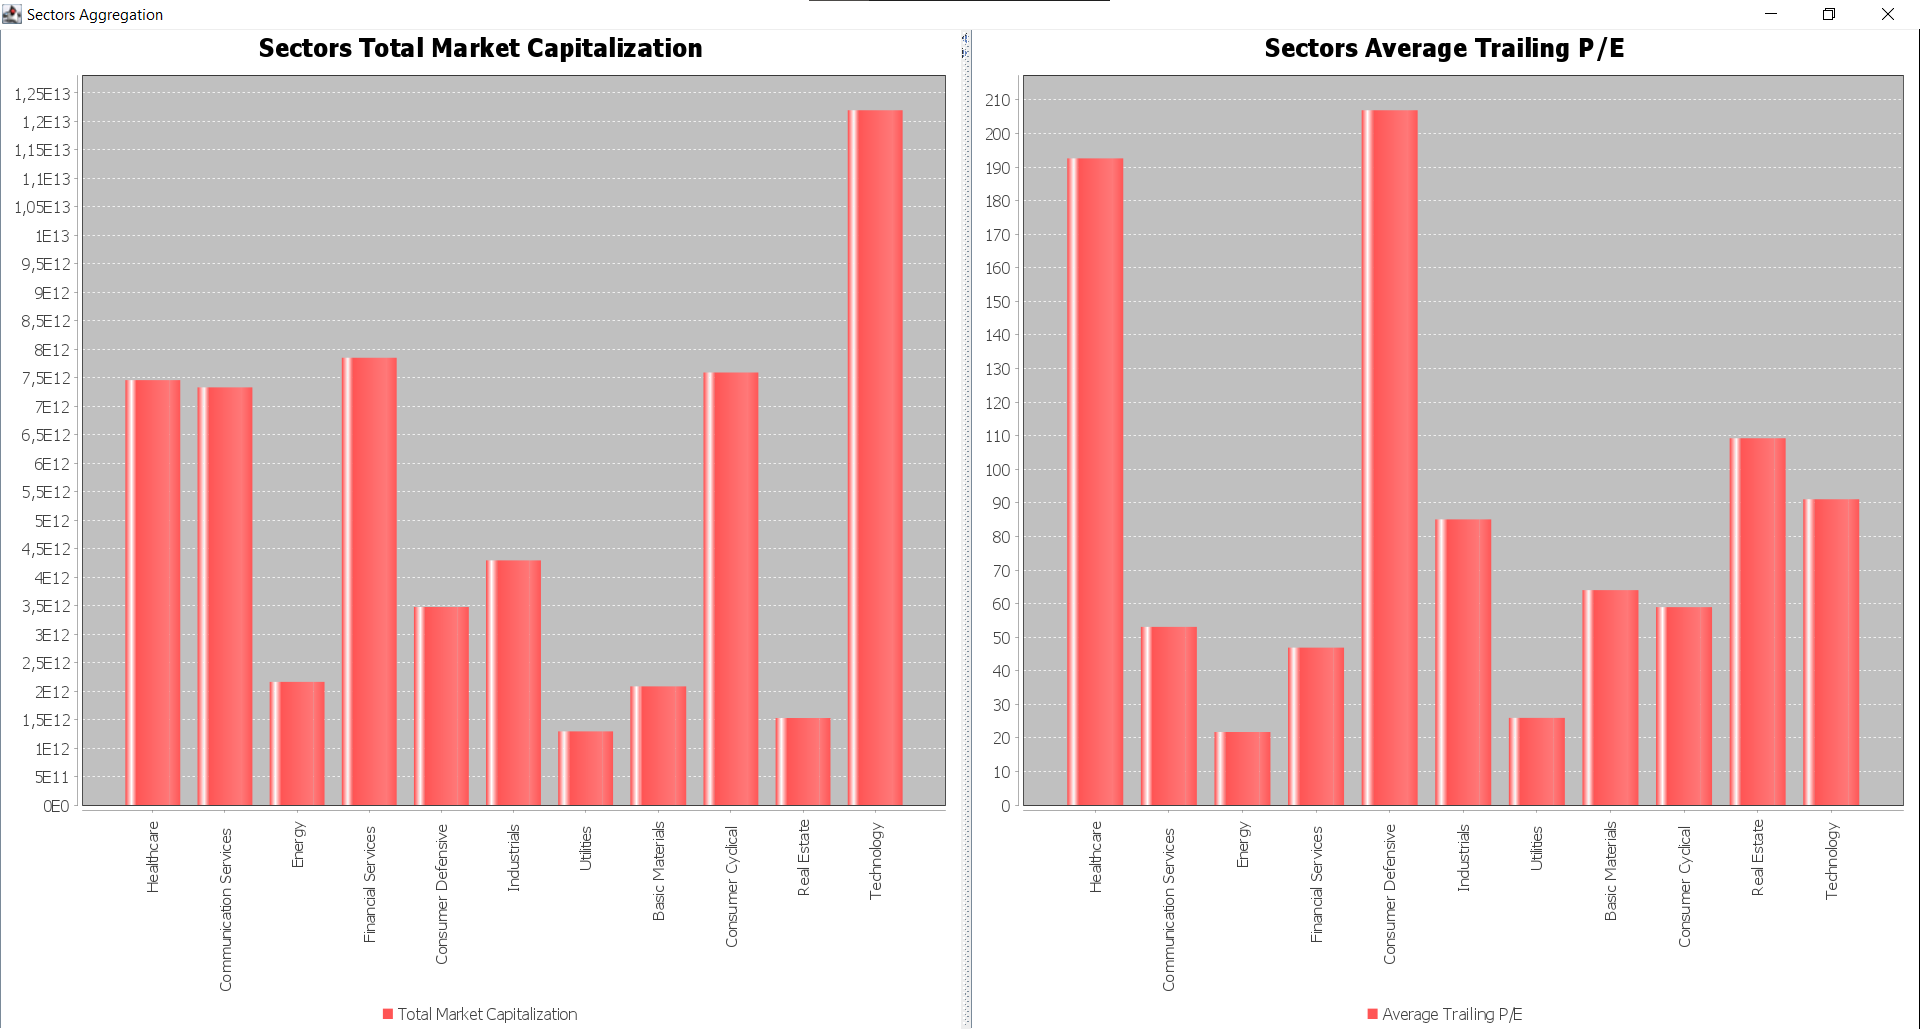
\includegraphics[scale=0.28]{img/user_manual/sector_aggregation.png}\\
}

\begin{lstlisting}[basicstyle=\footnotesize\ttfamily,language={},numbers=left,keepspaces=true,tabsize=4,
numberstyle=\footnotesize,numbersep=8pt,frame=single]
> sector-search
Sector Name: Energy
[ BROG, PSXP, KOS, GMLP, CLMT, NCSM, PFIE, CCLP, NGS, WES, ENSV, FTSI, AXAS, EC, DEN, TTI, NBLX, E, GTE, PSX, PED, NNA, VVV, PVL, AR, HP, CEQP, MUR, DK, RTLR, LEU, NGL, NFG, PTEN, MMLP, PAGP, NESR, NR, PBFX, TRMD, BKR, NOG, ... ]
\end{lstlisting}

The search by country is similar to the search by sector: it also opens two bar charts with aggregated data by country and returns a list of the symbols of all the stocks belonging to the specified country.
\begin{lstlisting}[basicstyle=\footnotesize\ttfamily,language={},numbers=left,keepspaces=true,tabsize=4,
numberstyle=\footnotesize,numbersep=8pt,frame=single]
> country-search
Country Name: Italy
[ E, NTZ, KLR, RACE, ]
\end{lstlisting}
\subsection{View stock}

The \texttt{view-stock} option allows the user to see the evolution of a stock in the market for a specific time range.\\
It asks the user for the stock symbol, the start and end dates and the day granularity, and then shows both a candlestick chart and a line chart of that stock for the desired time interval, along with printing all the information about that stock.

\begin{lstlisting}[basicstyle=\footnotesize\ttfamily,language={},numbers=left,keepspaces=true,tabsize=4,
numberstyle=\footnotesize,numbersep=8pt,frame=single]
> view-stock
Ticker Symbol: TSLA
Start Date [YYYY-MM-DD]: 2021-01-01
End Date [YYYY-MM-DD]: 2021-01-10
Days granularity: 1
Short Name: Tesla, Inc.
Long Name: Tesla, Inc.
Symbol: TSLA
Quote type: EQUITY
Market capitalization: 8.00041992192E11
PE ratio: 1265.3346
Market: us_market
Exchange timezone short name: EST
Exchange timezone name: America/New_York
Sector: Consumer Cyclical
Industry: Auto Manufacturers
Currency: USD
Location:  3500 Deer Creek Road Palo Alto CA United States
650-681-5000
Logo URL: https://logo.clearbit.com/tesla.com
Website: http://www.tesla.com
Long business summary:
Tesla, Inc. designs, develops, manufactures, leases, and sells electric
vehicles, and energy [...]
\end{lstlisting}

\hfill \break
{\centering
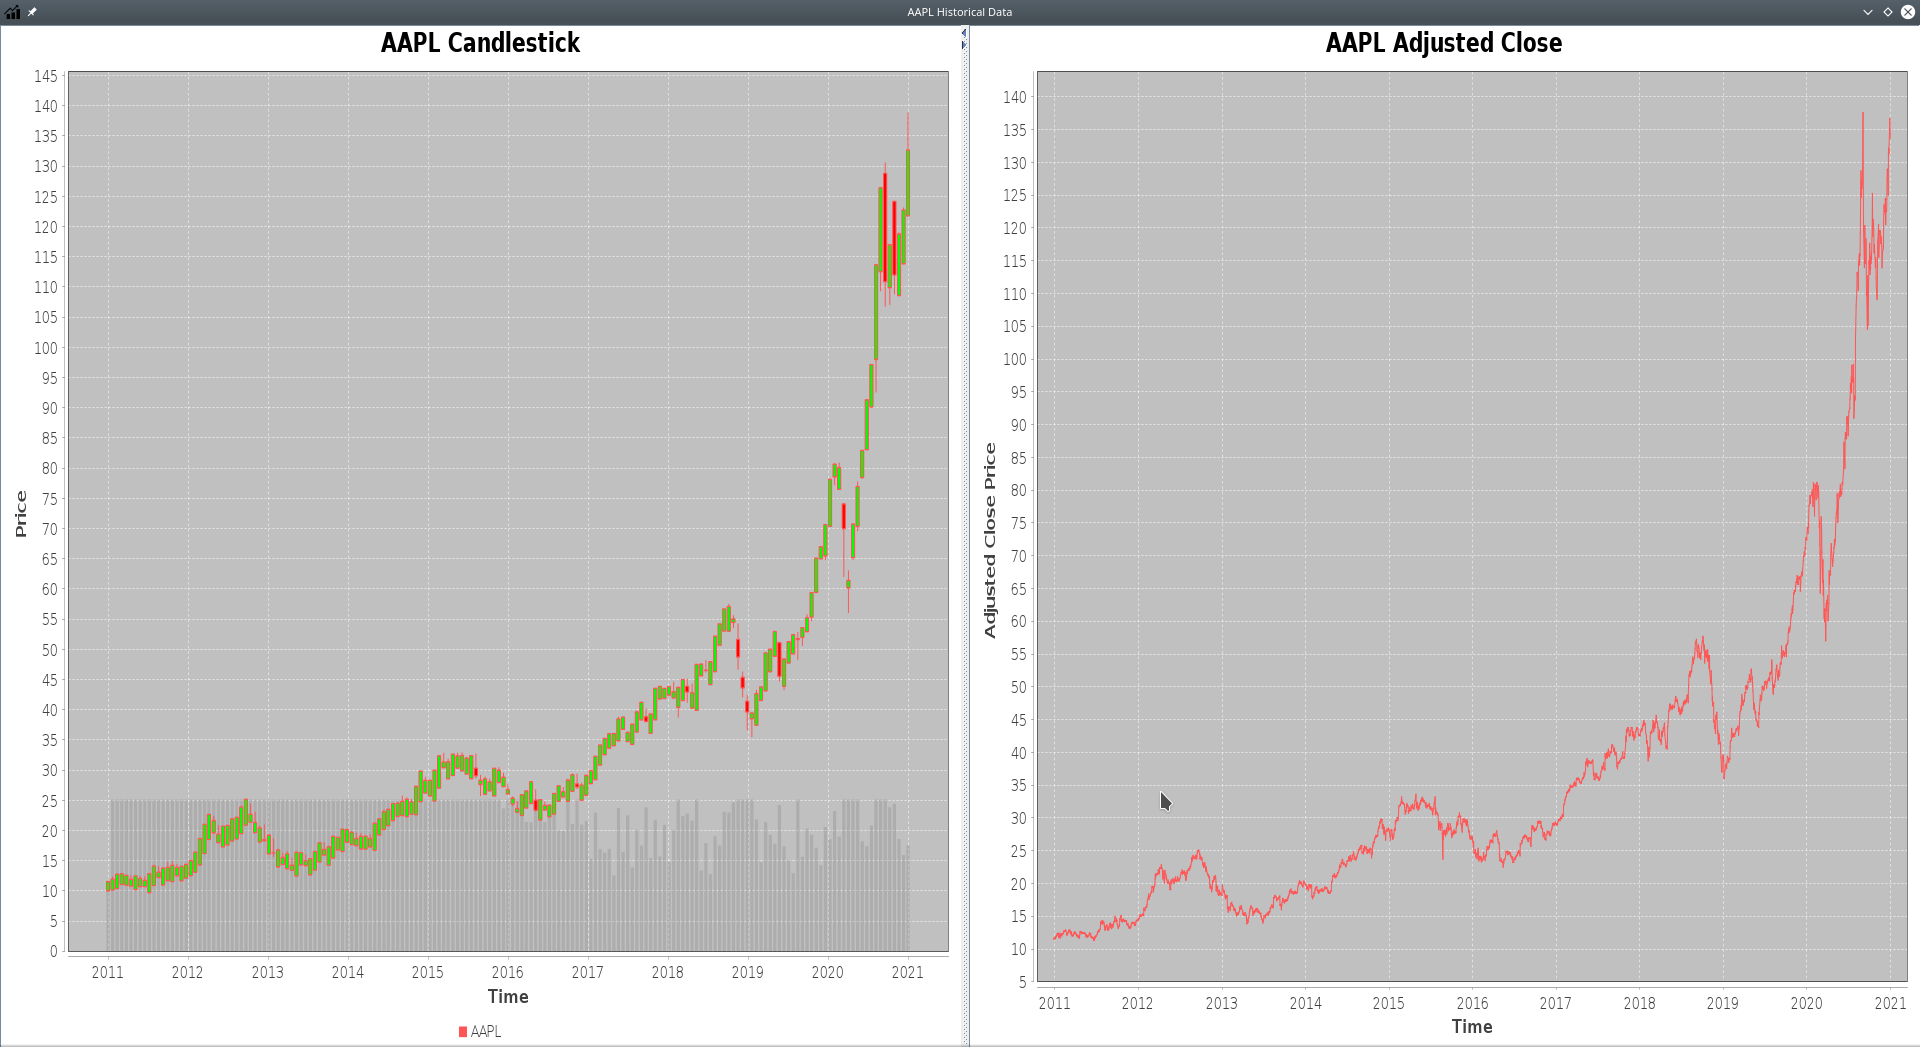
\includegraphics[scale=0.32]{img/user_manual/view_stock.png}\\
}

\subsection{Create portfolio}
The \texttt{create-portfolio} option allows the user create a new portfolio and insert stocks into it.\\
The user is first required to insert a name for the new portfolio and then to type a list of comma-separated symbols of the stocks they wish to insert in the portfolio.

\begin{lstlisting}[basicstyle=\footnotesize\ttfamily,language={},numbers=left,keepspaces=true,tabsize=4,
numberstyle=\footnotesize,numbersep=8pt,frame=single]
> create-portfolio
Portfolio name: Portfolio1
Ticker Symbols [comma separated]: TSLA, MSFT, RACE
Portfolio created correctly.

\end{lstlisting}

\subsection{List portfolios}
The \texttt{list-portfolios} option shows the user a list of all their portfolios and the stocks each one of them is made of.\\

\begin{lstlisting}[basicstyle=\footnotesize\ttfamily,language={},numbers=left,keepspaces=true,tabsize=4,
numberstyle=\footnotesize,numbersep=8pt,frame=single]
> list-portfolios
Portfolio1: [ TSLA, MSFT, RACE, ]
FAANG: [ FB, AAPL, AMZN, NFLX, GOOGL, ]
\end{lstlisting}

\subsection{View portfolio}
The \texttt{view-portfolio} option allows the user to view the composition of one of their portfolios. It prompts the user for the name of the portfolio to be viewed and then shows a pie chart of the portfolio.\\

{\centering
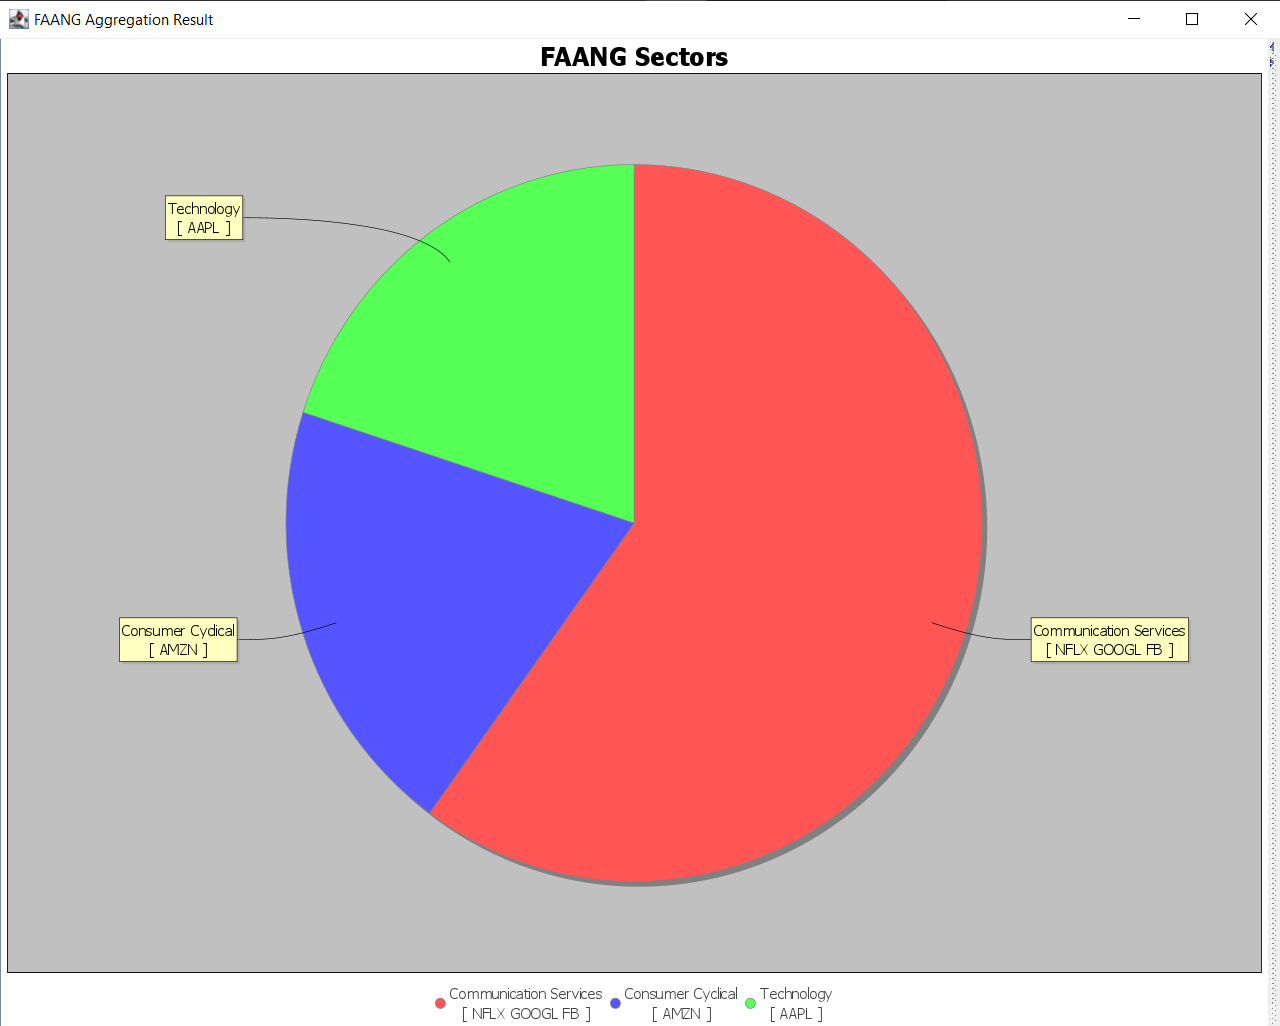
\includegraphics[scale=0.32]{img/user_manual/view_portfolio.png}\\
}

\subsection{Simulate portfolio}
TODO

\subsection{Delete portfolio}
The \texttt{delete-portfolio} option allows the user to delete one of their portfolios. It prompts the user for the name of the portfolio to be deleted and then it deletes the portfolio.

\section{StockSim Client Admin Mode}

After launching the application in \textit{admin} mode and logging in with admin credential, the following options are available:

\begin{lstlisting}[basicstyle=\footnotesize\ttfamily,language={},numbers=left,keepspaces=true,tabsize=4,
numberstyle=\footnotesize,numbersep=8pt,frame=single]
> login
Username: admin
Password: stocksim
Admin login executed correctly.
Welcome StockSim Admin.
Available Commands:

add-ticker			add a new ticker symbol to the database.
add-admin			create new admin account.                                                                                                                                                                     
remove-admin		delete admin account.                                                                                                                                                                         
remove-user			delete user account.                                                                                                                                                                          
logout				logout from current admin account.                                                                                                                                                            
quit				quit StockSim client.  
\end{lstlisting}

\subsection{Add ticker}
The \texttt{add-ticker} option allows an admin to add a ticker to the database, provided it exists in the Yahoo! Finance database.
The underlying function retrieves the data from YFinance and loads it into the application database.

\begin{lstlisting}[basicstyle=\footnotesize\ttfamily,,language={},numbers=left,keepspaces=true,tabsize=4,
numberstyle=\footnotesize,numbersep=8pt,frame=single]
> add-ticker
Ticker symbol: LSMSDB
Asset Profile created with success. Updating historical data.
Historical data updated with success.
\end{lstlisting}

\subsection{Add admin}
The \texttt{add-admin} option allows an admin to add other admin.
\begin{lstlisting}[basicstyle=\footnotesize\ttfamily,language={},numbers=left,keepspaces=true,tabsize=4,
numberstyle=\footnotesize,numbersep=8pt,frame=single]
> add-admin
Admin account name: John
Admin account surname: Doe
Admin account username: admin2
Admin account password: stocksim
New admin account created.
\end{lstlisting}

\subsection{Remove admin}

The \texttt{remove-admin} option allows an admin to remove another admin from their role.

\begin{lstlisting}[basicstyle=\footnotesize\ttfamily,language={},numbers=left,keepspaces=true,tabsize=4,
numberstyle=\footnotesize,numbersep=8pt,frame=single]
> remove-admin
Admin account username: admin2
Admin account password: stocksim
Admin account deleted.
\end{lstlisting}

\subsection{Remove user}
The \texttt{remove-user} option allows an admin to delete a user from the database.

\begin{lstlisting}[basicstyle=\footnotesize\ttfamily,language={},numbers=left,keepspaces=true,tabsize=4,
numberstyle=\footnotesize,numbersep=8pt,frame=single]
> remove-user
User account email: jsmith@example.com
User account deleted.
\end{lstlisting}


\end{document}
